\documentclass[11pt]{article} \usepackage{fullpage} \usepackage{graphicx} \usepackage{epstopdf} \usepackage{color} \usepackage{psfrag} \usepackage{pdfsync}\usepackage{indentfirst}\usepackage{subfigure}\usepackage{float}\usepackage[section]{placeins}
\usepackage{enumerate}
\usepackage{multirow}
\usepackage{amsfonts, fullpage, graphics} 
\usepackage{algorithm,algorithmic}
\usepackage{amsmath,amssymb,amsthm,bm,hyperref}
\usepackage{dsfont}
\usepackage[parfill]{parskip}
\usepackage[margin=1in]{geometry}
\newcommand{\Lagr}{\mathcal{L}}
\newcommand{\norm}[1]{\left\lVert#1\right\rVert}
\newcommand{\floor}[1]{\lfloor #1 \rfloor}
\newcommand{\todo}[1]{}
\renewcommand{\todo}[1]{{\color{red} TODO: {#1}}}
\newcommand\independent{\protect\mathpalette{\protect\independenT}{\perp}}
\newcommand{\obar}[1]{\mkern 1.5mu\overline{\mkern-1.5mu#1\mkern-1.5mu}\mkern 1.5mu}
\def\independenT#1#2{\mathrel{\rlap{$#1#2$}\mkern2mu{#1#2}}}
\newcommand{\rpm}{\sbox0{$1$}\sbox2{$\scriptstyle\pm$}
  \raise\dimexpr(\ht0-\ht2)/2\relax\box2 }
\usepackage{xspace}
\newcommand{\latex}{\LaTeX\xspace}
\setlength{\parindent}{2em}

\usepackage{listings}
\usepackage{color} %red, green, blue, yellow, cyan, magenta, black, white
\definecolor{mygreen}{RGB}{28,172,0} % color values Red, Green, Blue
\definecolor{mylilas}{RGB}{170,55,241}
\DeclareMathOperator{\E}{\mathbb{E}}
\DeclareMathOperator*{\argmax}{arg\,max}
\DeclareMathOperator*{\argmin}{arg\,min}

\begin{document}

{\parindent 0pt \begin{tabular}[t]{l} 16-720 Computer Vision \\ Spring 2020 \end{tabular}}%  \hfill XX/XX/14 \vskip 0.2in }
\parindent 0pt \parskip 8pt
\begin{center} \large\bf Homework 6 \end{center}
\begin{center} \large\bf Zongwen Mu, Andrew ID: zongwenm \end{center}
\bigskip


\section{Calibrated Photometric Stereo}

\setlength{\parindent}{2em}  

\paragraph{a}~{}

In $n$-dot-$l$ lighting, the surface radiance is 
\begin{equation}
	L = \frac{\rho_d}{\pi}I\cos\theta_i
\end{equation}

where $\cos\theta_i$ is equal to $\vec{n}\cdot\vec{s}$, since angle between $l$ and $n$ is defined as $\theta_i$, we have:
\begin{figure}[H]
\centering
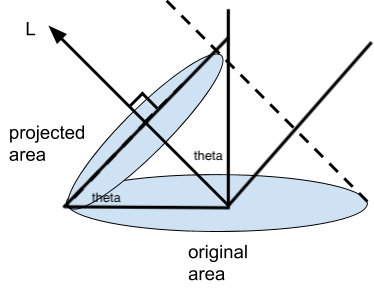
\includegraphics[width=0.4\textwidth]{results/projected_1.png}
\caption{Projection}
\end{figure}

In this case, we can see that the projected area's projection in original area (the actual area) equals to (projected area $* \cos\theta_i$).

And since surface appears equally bright for all directions, the viewing direction does not matter in this case.

\paragraph{b}~{}

Rendering results are shown below:
\begin{figure}[H]
\centering
\subfigure[]{
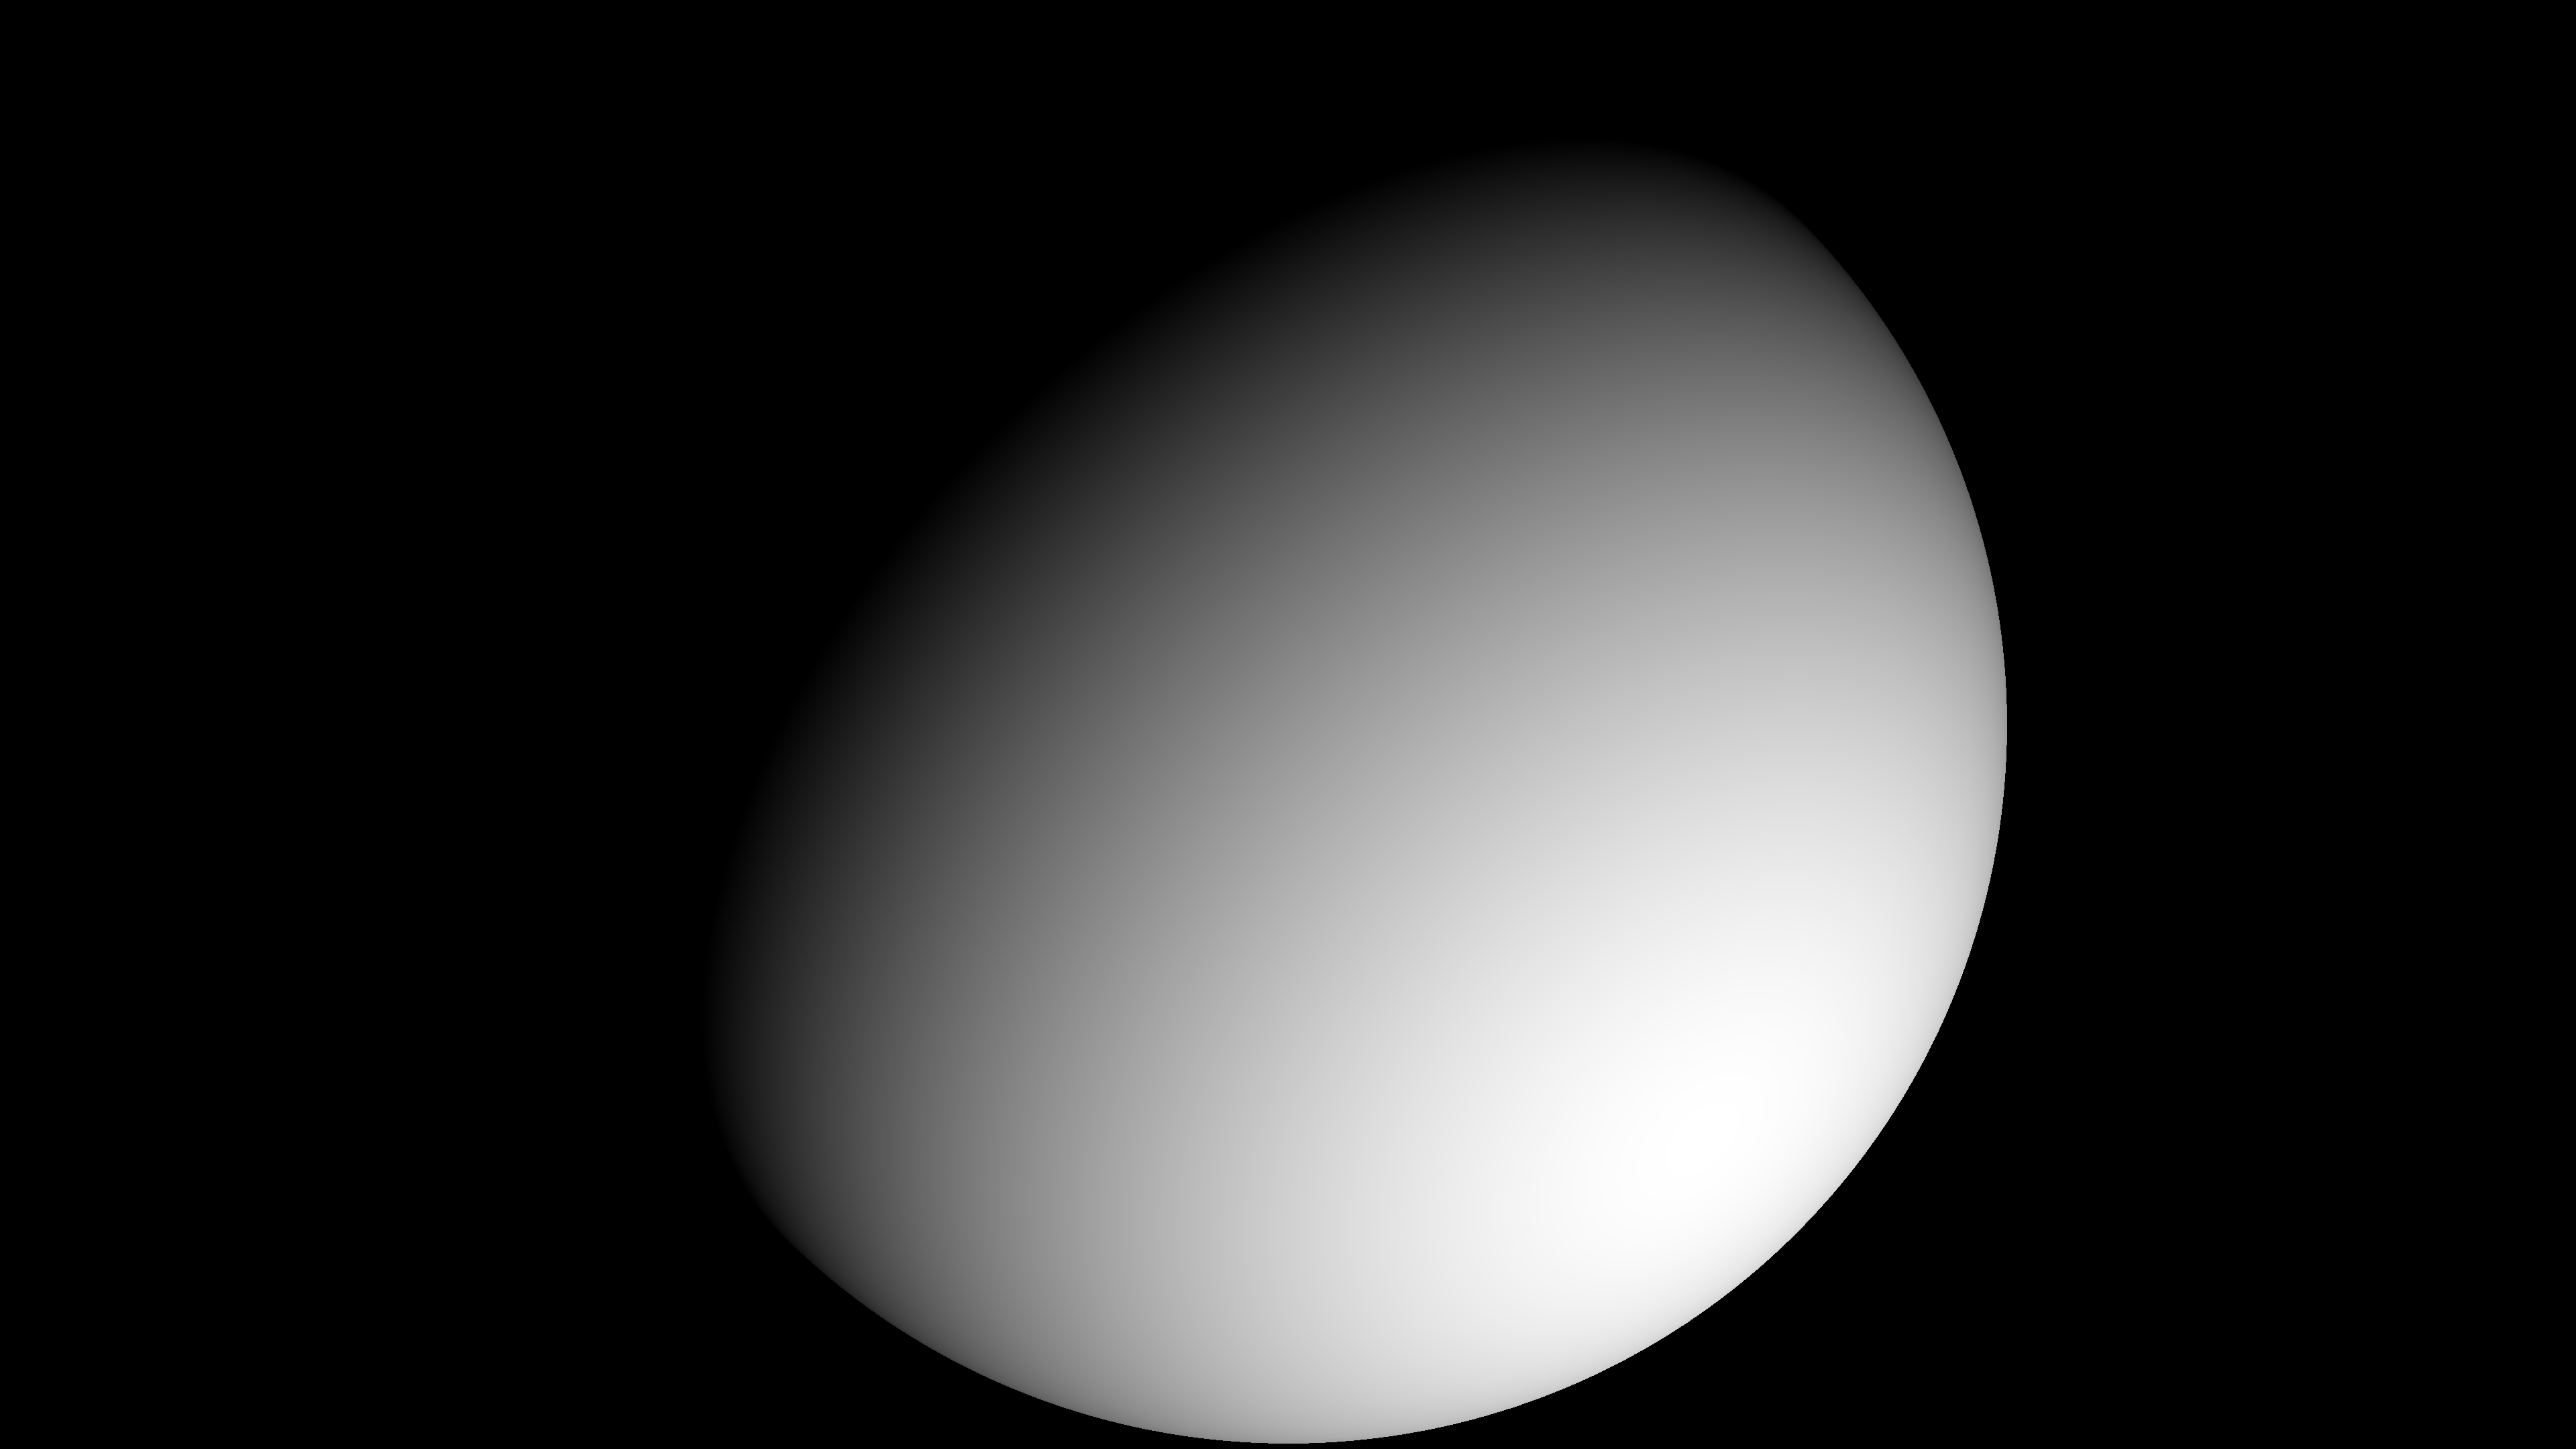
\includegraphics[width=0.3\textwidth]{results/q1b_1.png}}
\subfigure[]{
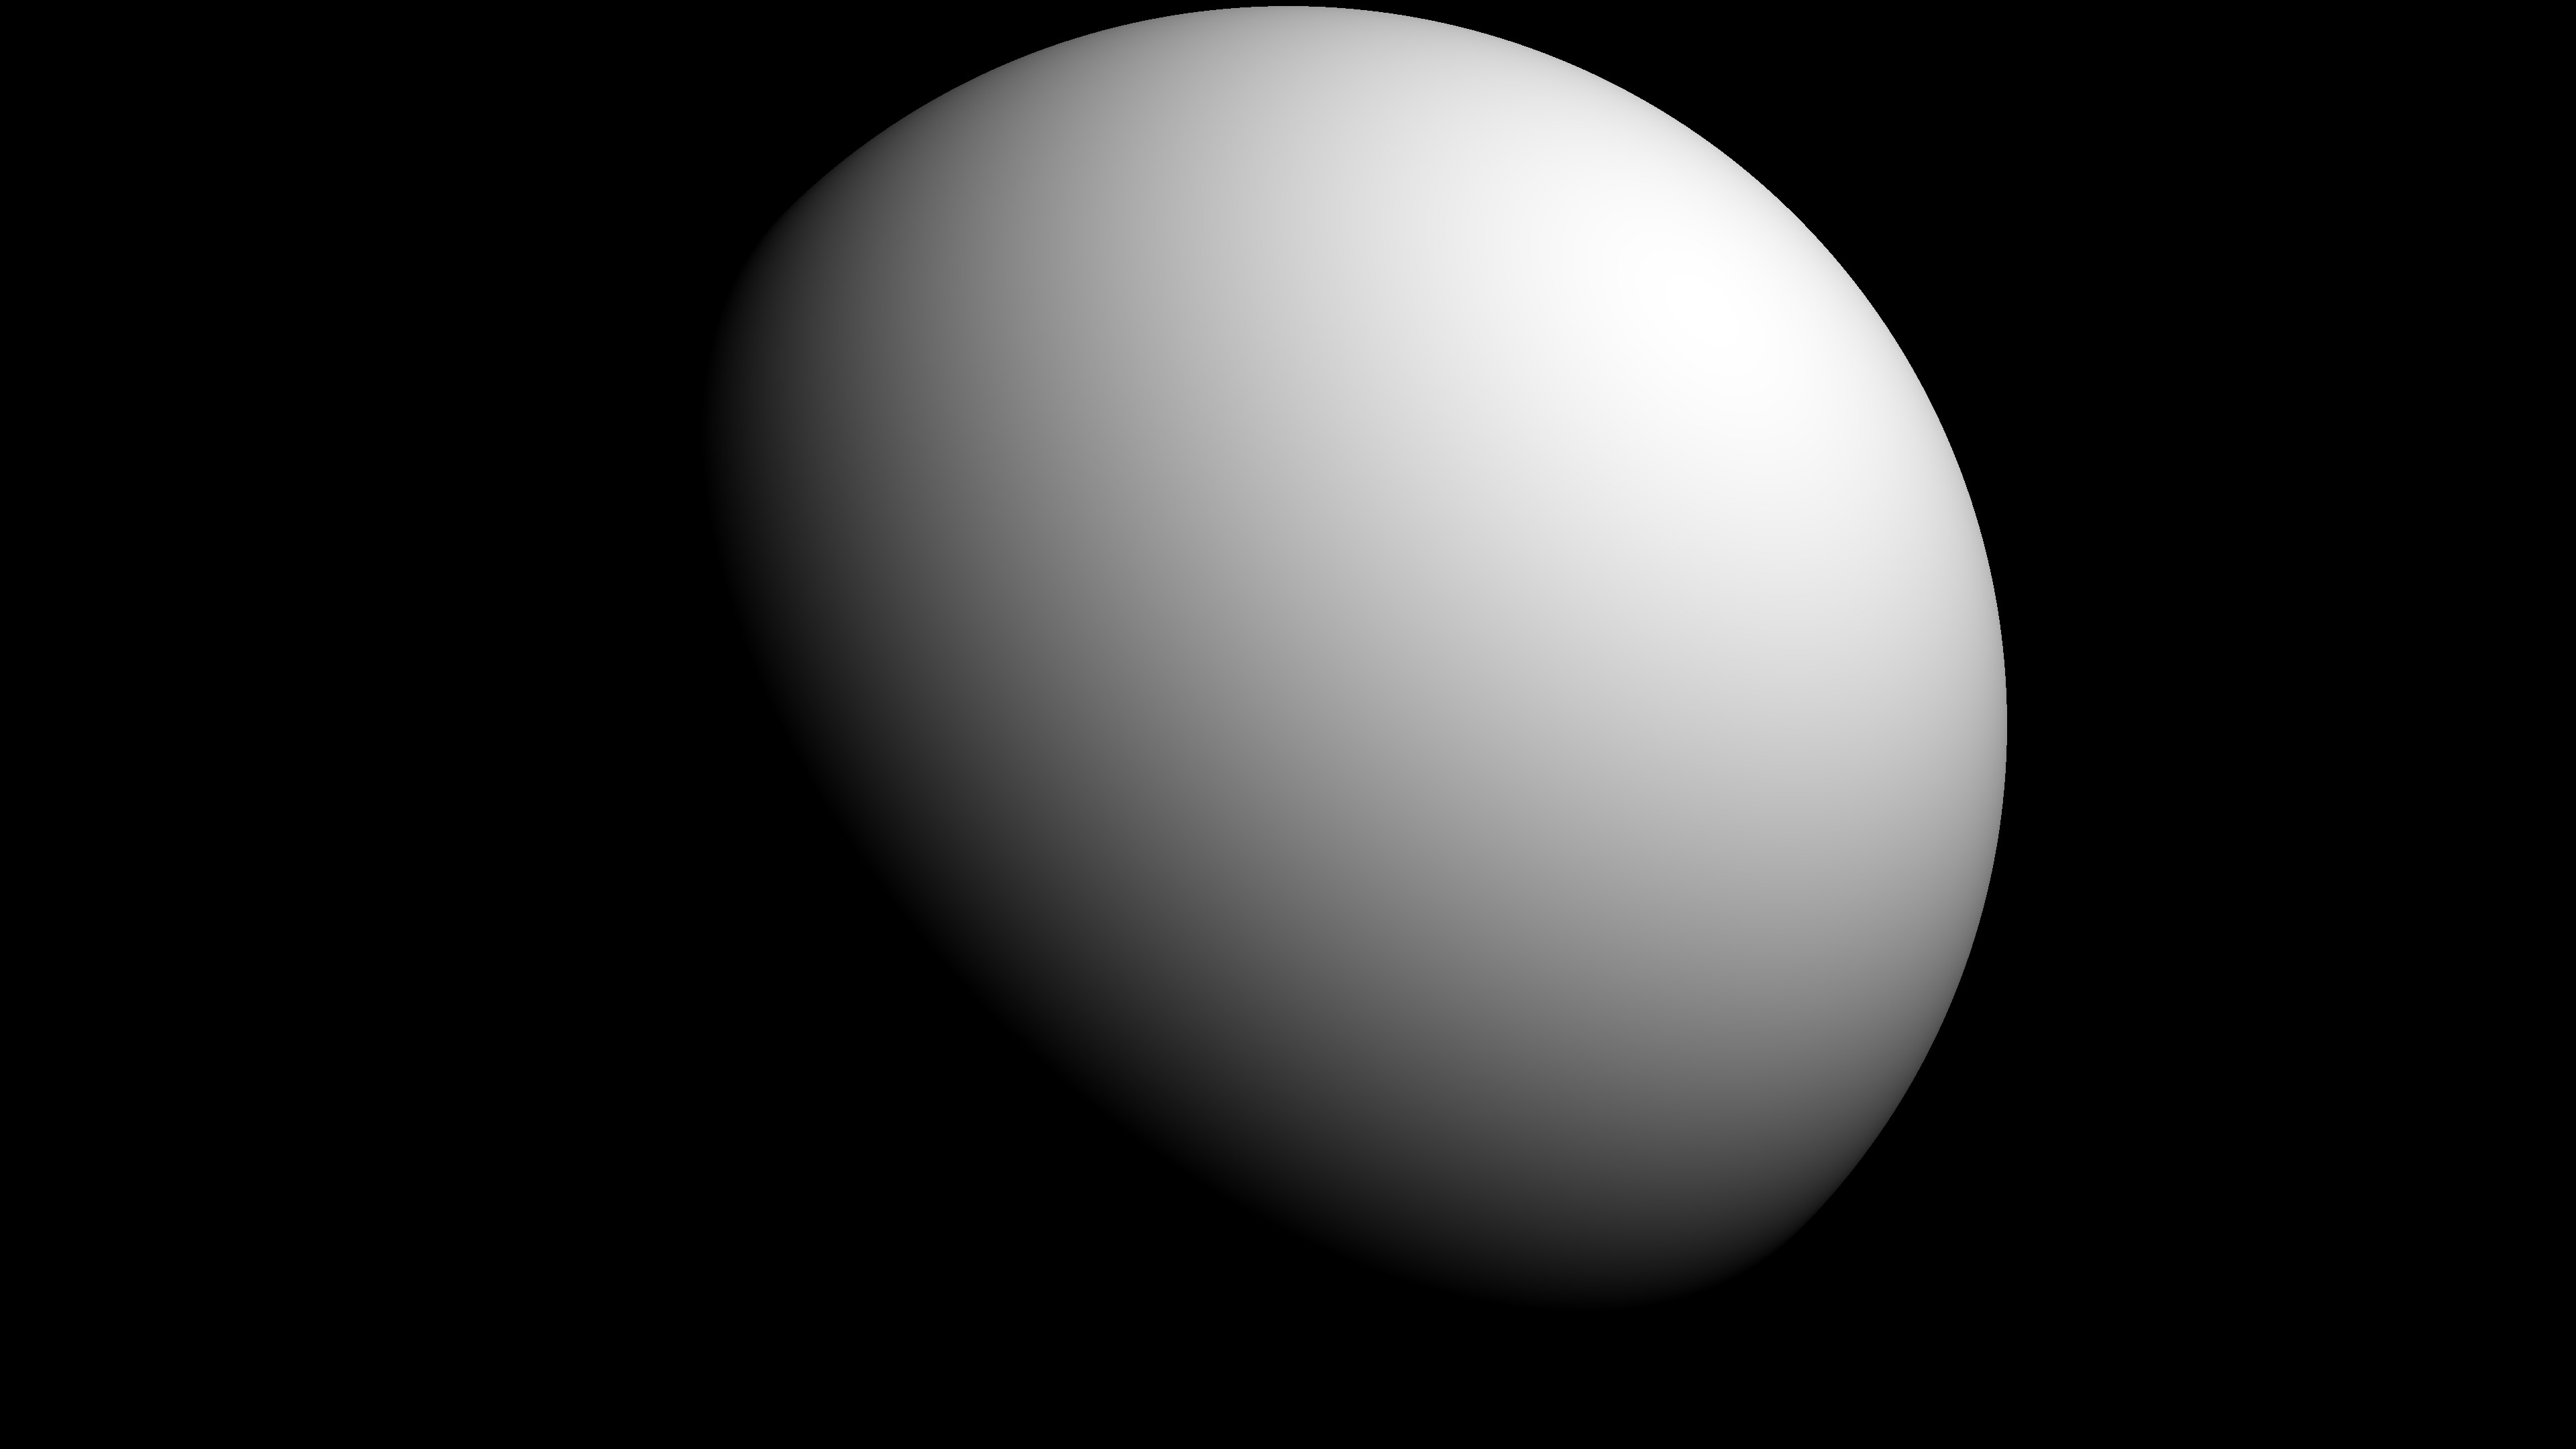
\includegraphics[width=0.3\textwidth]{results/q1b_2.png}}
\subfigure[]{
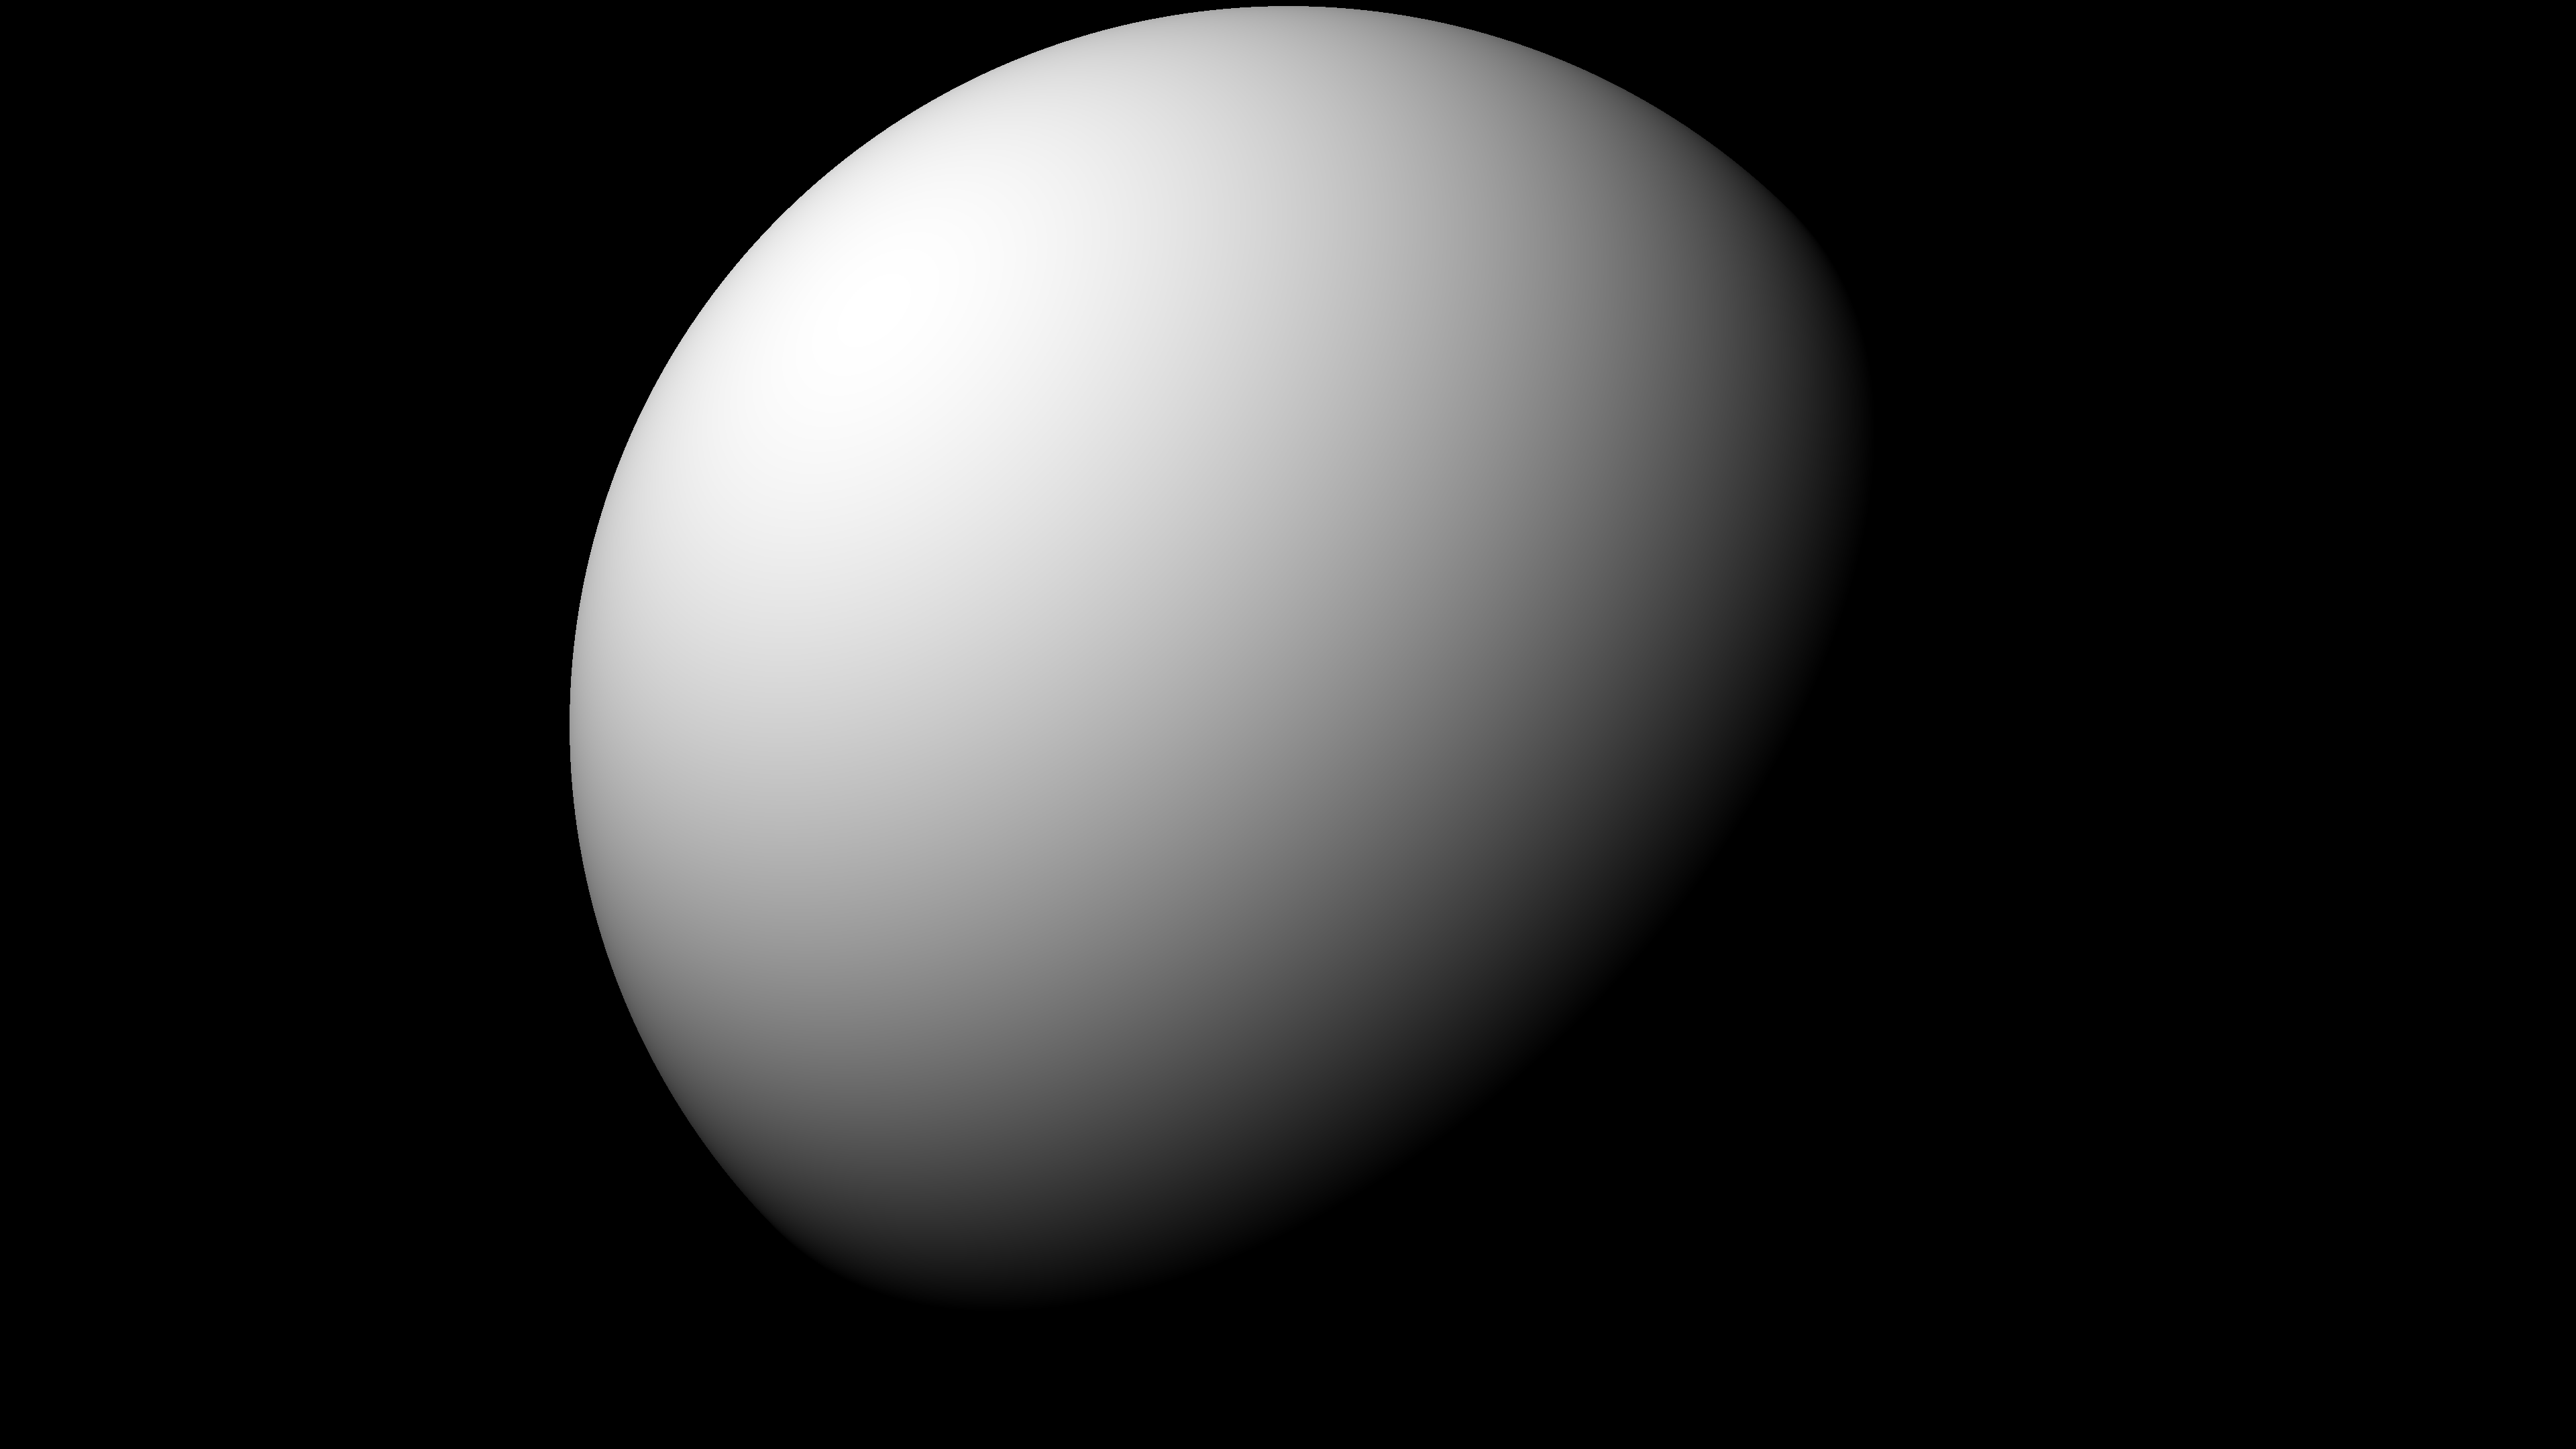
\includegraphics[width=0.3\textwidth]{results/q1b_3.png}}
\caption{Rendering results}
\end{figure}

\paragraph{d}~{}

In this case, $\bold{n}$ is in $3d$ coordinates, which means we will need $3$ light sources from different directions to determine it. Therefore, with $3$ different light sources, the intensity matrix $\bold{I}$ should have rank $3$.

However, when doing SVD for matrix $\bold{I}$ obtained from previous question, the singular values are $\begin{bmatrix} 66066.781 & 7845.767 & 5478.122 & 1666.105 &1265.811 & 1000.857 & 815.402 \end{bmatrix}$, which tend to have rank $7$ and do not agree with rank-$3$ requirement.

This may be caused by the non-idealities like blurring in image capture process. Therefore, we may need more captures images lighted from different directions to help in reconstruction.

\paragraph{e}~{}

Consider a linear system $\bold{Ax} = \bold{y}$, in which we could solve $\bold{x}$ as $\bold{A^{-1}y}$. We could solve $\bold{B}$ by:
\begin{equation}
	\bold{B} = \bold{\left(L^{\mathbf{T}}\right)^{-1}I}
\end{equation}

But in this case, $\bold{L}$ is not a square matrix, so we can't solve $\bold{\left(L^{\mathbf{T}}\right)^{-1}}$ directly, so we have:
\begin{align}
	\bold{\left(LL^{\mathbf{T}}\right)^{-1}} & = \bold{\left(L^{\mathbf{T}}\right)^{-1}L^{-1}} \\
	\bold{\left(L^{\mathbf{T}}\right)^{-1}} & = \bold{\left(LL^{\mathbf{T}}\right)^{-1}}\bold{L}
\end{align}

Therefore, we could solve $\bold{B}$ by:
\begin{equation}
	\bold{B} = \bold{\left(LL^{\mathbf{T}}\right)^{-1}\bold{L}I}
\end{equation}

While compared with linear model, $\bold{A}$ is equal to $\bold{LL^{\mathbf{T}}}$ and $\bold{y}$ is equal to $\bold{LI}$.

\paragraph{f}~{}

\begin{figure}[H]
\centering
\subfigure[Albedo Image]{
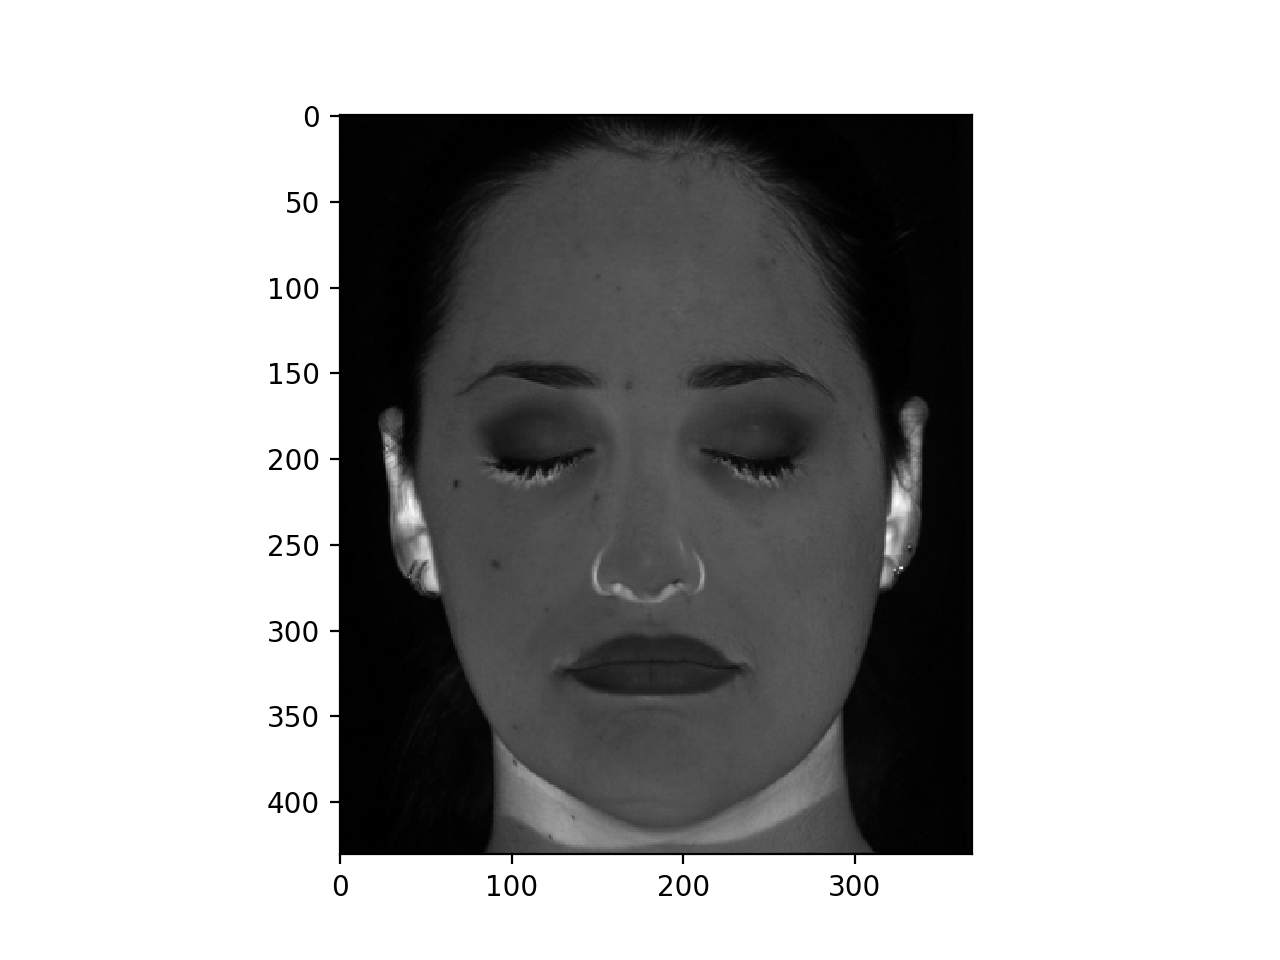
\includegraphics[width=0.4\textwidth]{results/q1e_albedo.png}}
\subfigure[Normal Image]{
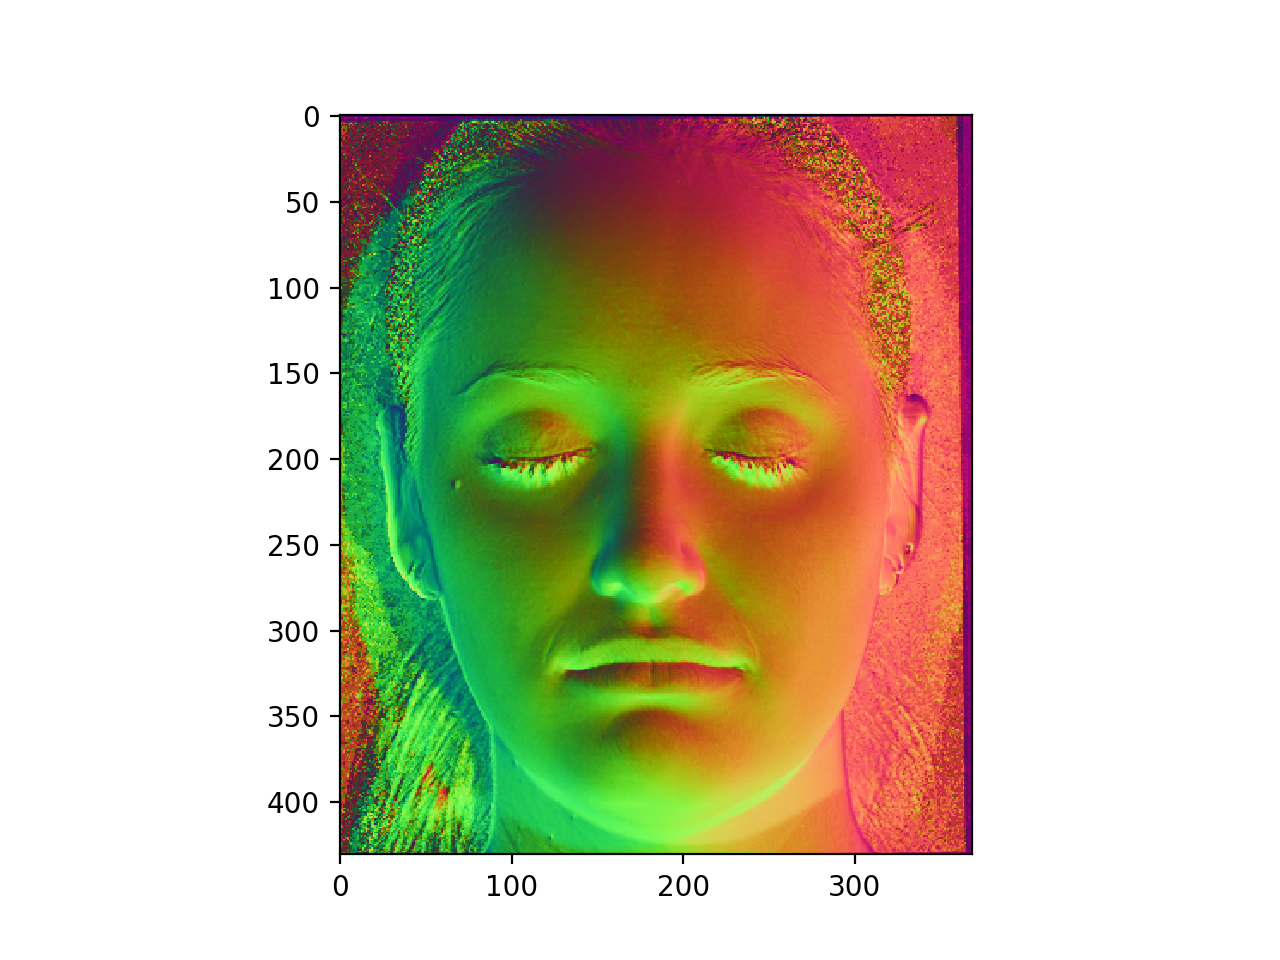
\includegraphics[width=0.4\textwidth]{results/q1e_normal.png}}
\caption{Albedos and Normals}
\end{figure}

\paragraph{Comment:}~{}

Albedo performed poorly at pixels around nostrils, neck and ears, this is because our n-dot-l model assumes directional lighting from one source and does not account for shadows. Therefore, if some parts are hidden under shadows, we will probably lose information to reconstruct normals.

\paragraph{g}~{}

For a depth problem, we have:
\begin{align}
	V_1 & = \left(1, 0, z_{x+1, y} - z_{x, y}\right) \\
	0 & = N \cdot V_1 \\
	& = n_1 + n_3\left(z_{x+1, y} - z_{x, y}\right)
\end{align}

Similarly, we have:
\begin{align}
	V_2 & = \left(1, 0, z_{x, y+1} - z_{x, y}\right) \\
	0 & = N \cdot V_2 \\
	& = n_2 + n_3\left(z_{x, y+1} - z_{x, y}\right)
\end{align}

Therefore:
\begin{align}
	\frac{\partial{f\left(x, y\right)}}{\partial{x}} & = -\frac{n_1}{n_3} \\
	\frac{\partial{f\left(x, y\right)}}{\partial{y}} & = -\frac{n_2}{n_3}
\end{align}

\paragraph{h}~{}

Gradient matrices:
\begin{align}
	g_x & = \begin{bmatrix} 1 & 1 & 1  \\ 1 & 1 & 1 \\ 1 & 1 & 1 \\ 1 & 1 & 1 \end{bmatrix} \\
	g_y & = \begin{bmatrix} 4 & 4 & 4 & 4 \\ 4 & 4 & 4 & 4 \\ 4 & 4 & 4 & 4 \end{bmatrix}
\end{align}

Reconstructed $g$ matrices from both way are the same:

\begin{equation}
	g = \begin{bmatrix} 1 & 2 & 3 & 4 \\ 5 & 6 & 7 & 8 \\ 9 & 10 & 11 & 12 \\ 13 & 14 & 15 & 16 \end{bmatrix}
\end{equation}

When gradients toward a specific direction is modified, the $g_x$ and $g_y$ would not be non-integrable, therefore, when we calculate gradients from both $x$ and $y$ directions in (g), there is the possibility that in some slope and edges the gradients will be non-integrable.

\paragraph{i}~{}

The surface plot is shown below:
\begin{figure}[H]
\centering
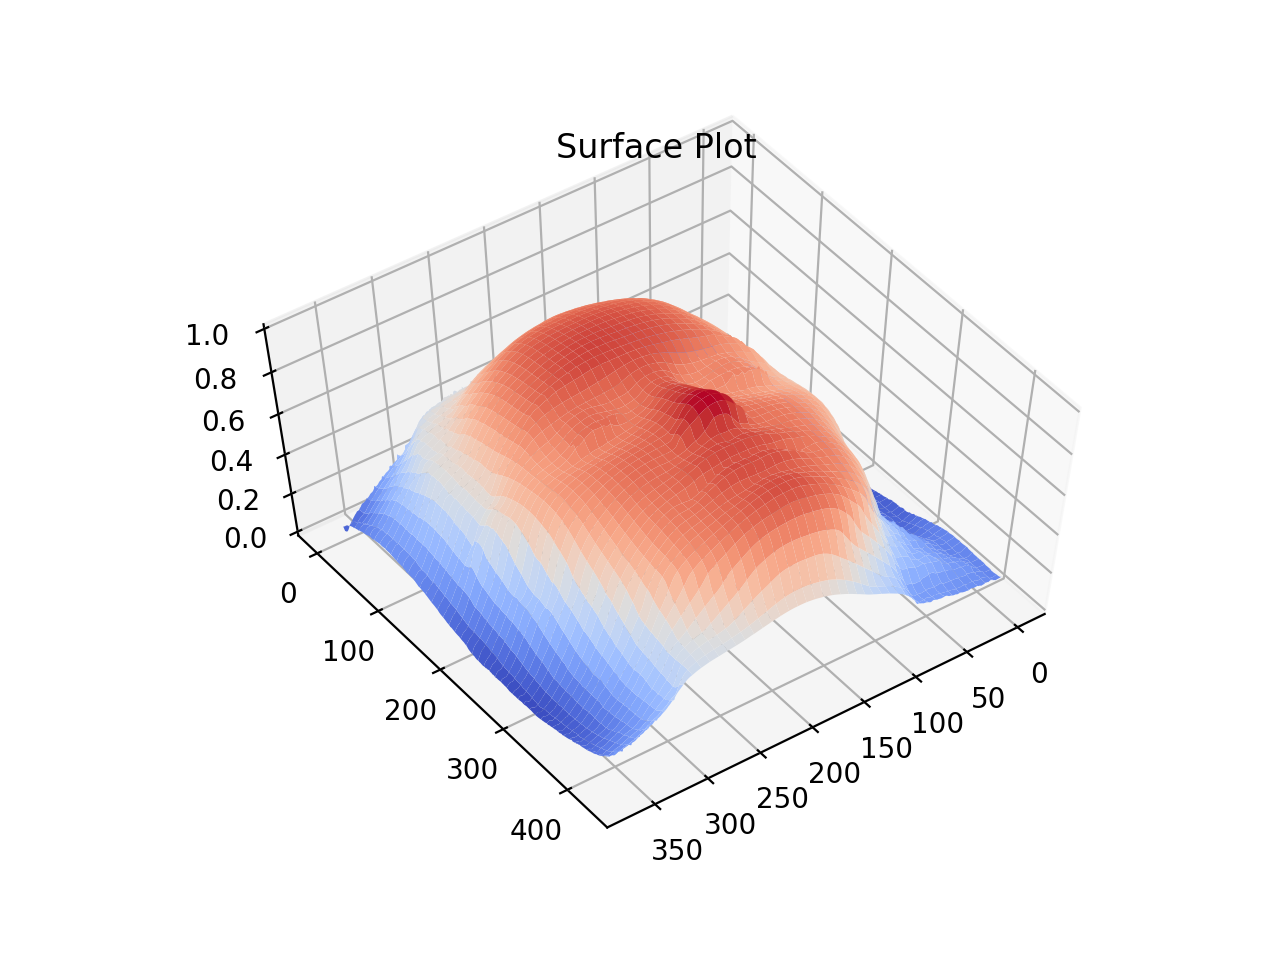
\includegraphics[width=0.8\textwidth]{results/q1i.png}
\caption{Surface Plot}
\end{figure}

\section{Uncalibrated Photometric Stereo}

\paragraph{a}~{}

For singular value decomposition we have $\bold{M} = \bold{U\Sigma V^\mathbf{T}}$, therefore, we could do same thing to matrix $\bold{I}$:
\begin{equation}
	\bold{I} = \bold{U\Sigma V^{\mathbf{T}}}
\end{equation}

In this case, $\bold{I}$ has a dimension of $7\times P$, so $\bold{U}$ is $7\times7$ and $\bold{V}$ is $P\times P$. Set all singular values except top $k$ from $\Sigma$ to $0$ and choose top $3$ vector from $\bold{U}$ as $\bold{L}$ and top $3$ vector from $\bold{V}$ as $\bold{B}$.

\paragraph{b}~{}

Visualized result is shown below:
\begin{figure}[H]
\centering
\subfigure[Albedo Image]{
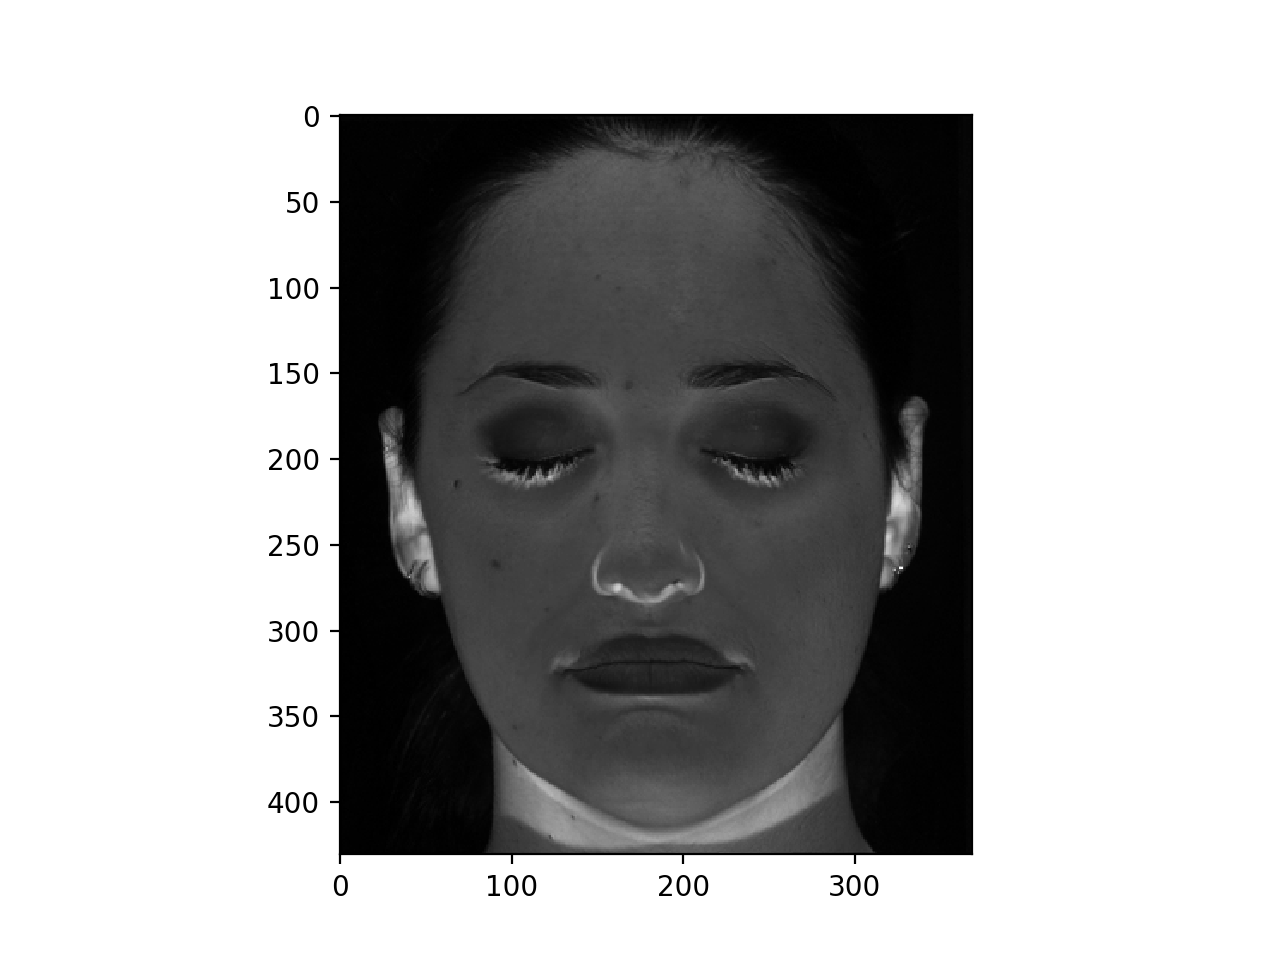
\includegraphics[width=0.4\textwidth]{results/q2b_albedo.png}}
\subfigure[Normal Image]{
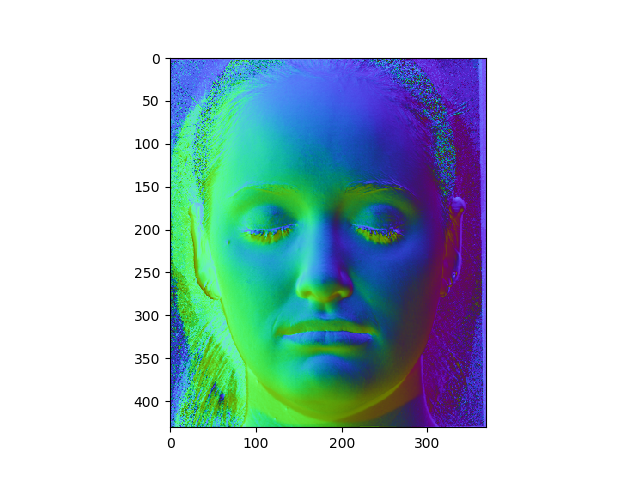
\includegraphics[width=0.4\textwidth]{results/q2b_normal.png}}
\caption{Albedos and Normals}
\end{figure}

\paragraph{c}~{}

Ground Truth lighting $\bold{L_0}$ is $\begin{bmatrix} -0.1418 & 0.1215 & -0.069 & 0.067 & -0.1627 & 0 & 0.1478 \\ -0.1804 & -0.2026 & -0.0345 & -0.0402 & 0.122 & 0.1194 & 0.1209 \\ -0.9267 & -0.9717 & -0.838 & -0.9772 & -0.979 & -0.9648 & -0.9713 \end{bmatrix}$, while estimated $\hat{\bold{L}}$ is $\begin{bmatrix} -0.3556 & 0.3549 & 0.6277 & -0.5443 & -0.1553 & 0.1480 & 0.1065 \\ -0.3984 & -0.6284 & 0.3992 & 0.4232 & -0.3141 & 0.0145 & 0.0957 \\ -0.3255 & 0.1789 & 0.1064 & 0.2528 & 0.2877 & 0.1618 & -0.8233 \end{bmatrix}$, which is quite different. Normalizing $\hat{\bold{L}}$ and $\bold{B}$ and multiplying $\hat{\bold{B}}$ with a $\bold{G}$ matrix with form $\begin{bmatrix} 1 & 0 & 0 \\ 0 & 1 & 0 \\ \mu & \nu & \lambda \end{bmatrix}$ could change $\bold{B}$ without changing rendering results.

\paragraph{d}~{}

Reconstructed result is shown below, but it does not look like a face:
\begin{figure}[H]
\centering
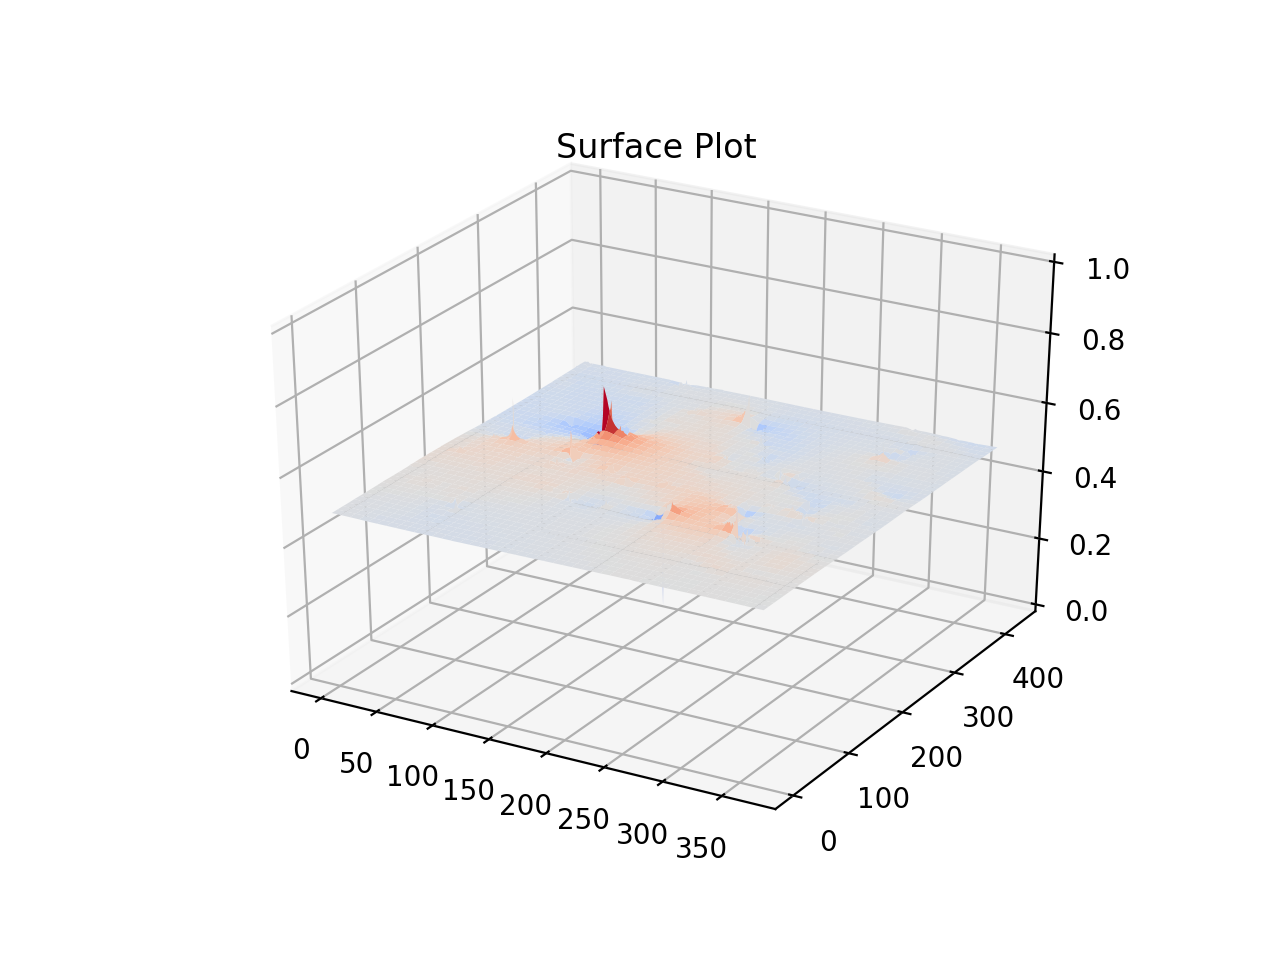
\includegraphics[width=0.8\textwidth]{results/q2d.png}
\caption{Surface Plot}
\end{figure}

\paragraph{e}~{}

Reconstructed results are shown below:
\begin{figure}[H]
\centering
\subfigure[Viewpoints 1]{
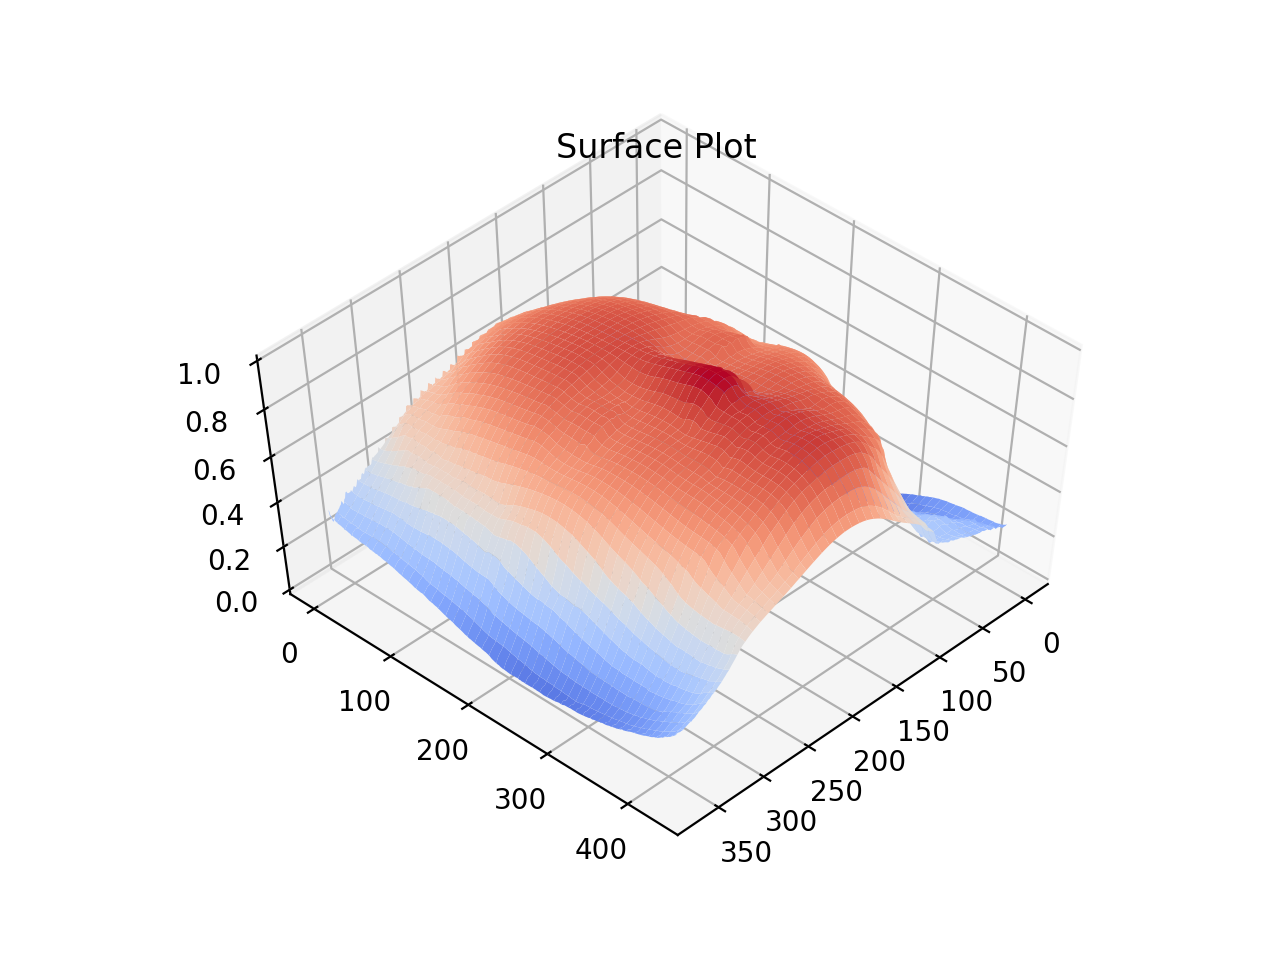
\includegraphics[width=0.3\textwidth]{results/q2e_1.png}}
\subfigure[Viewpoints 2]{
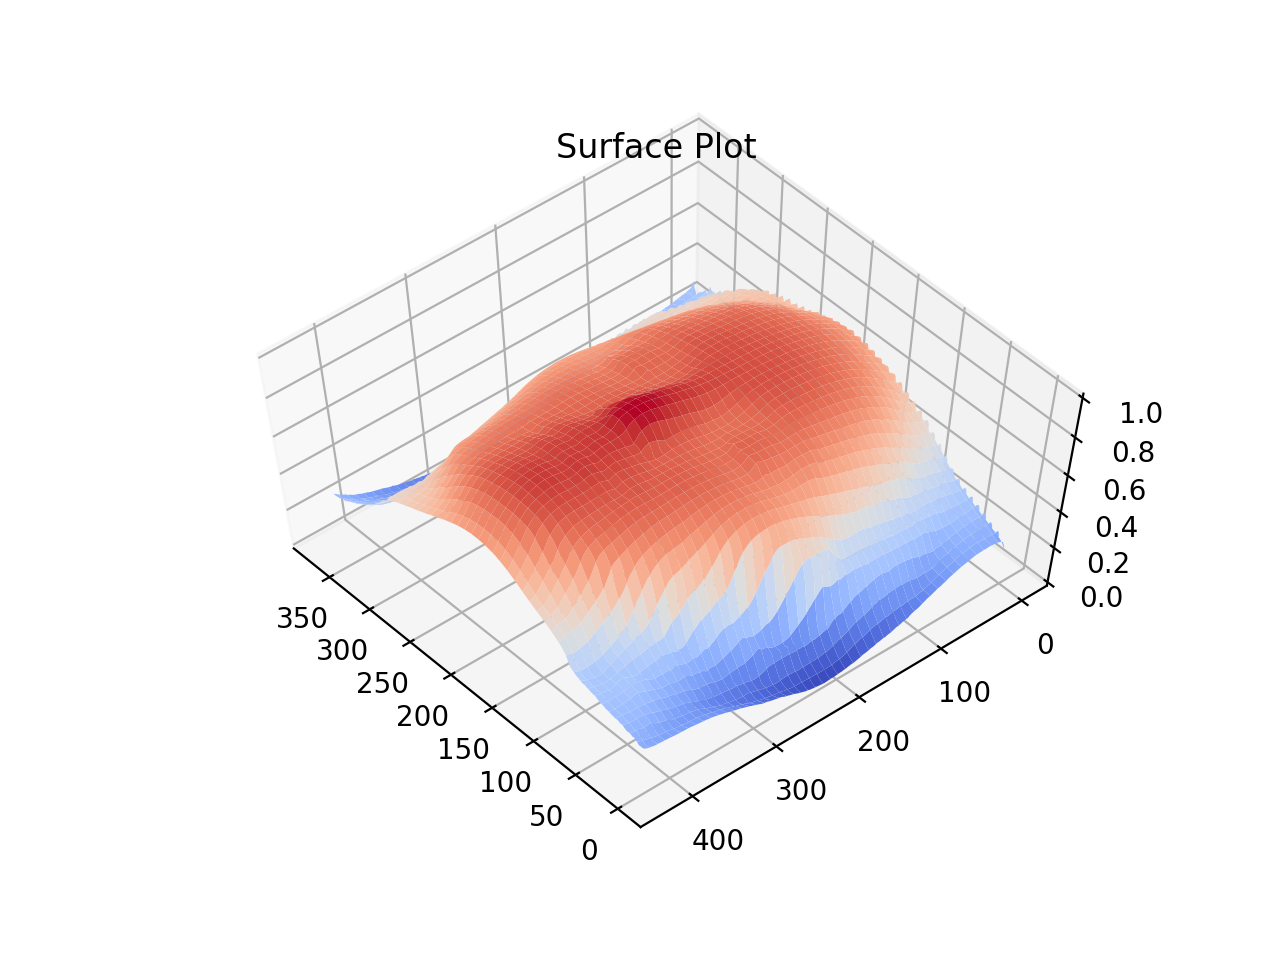
\includegraphics[width=0.3\textwidth]{results/q2e_2.png}}
\subfigure[Viewpoints 3]{
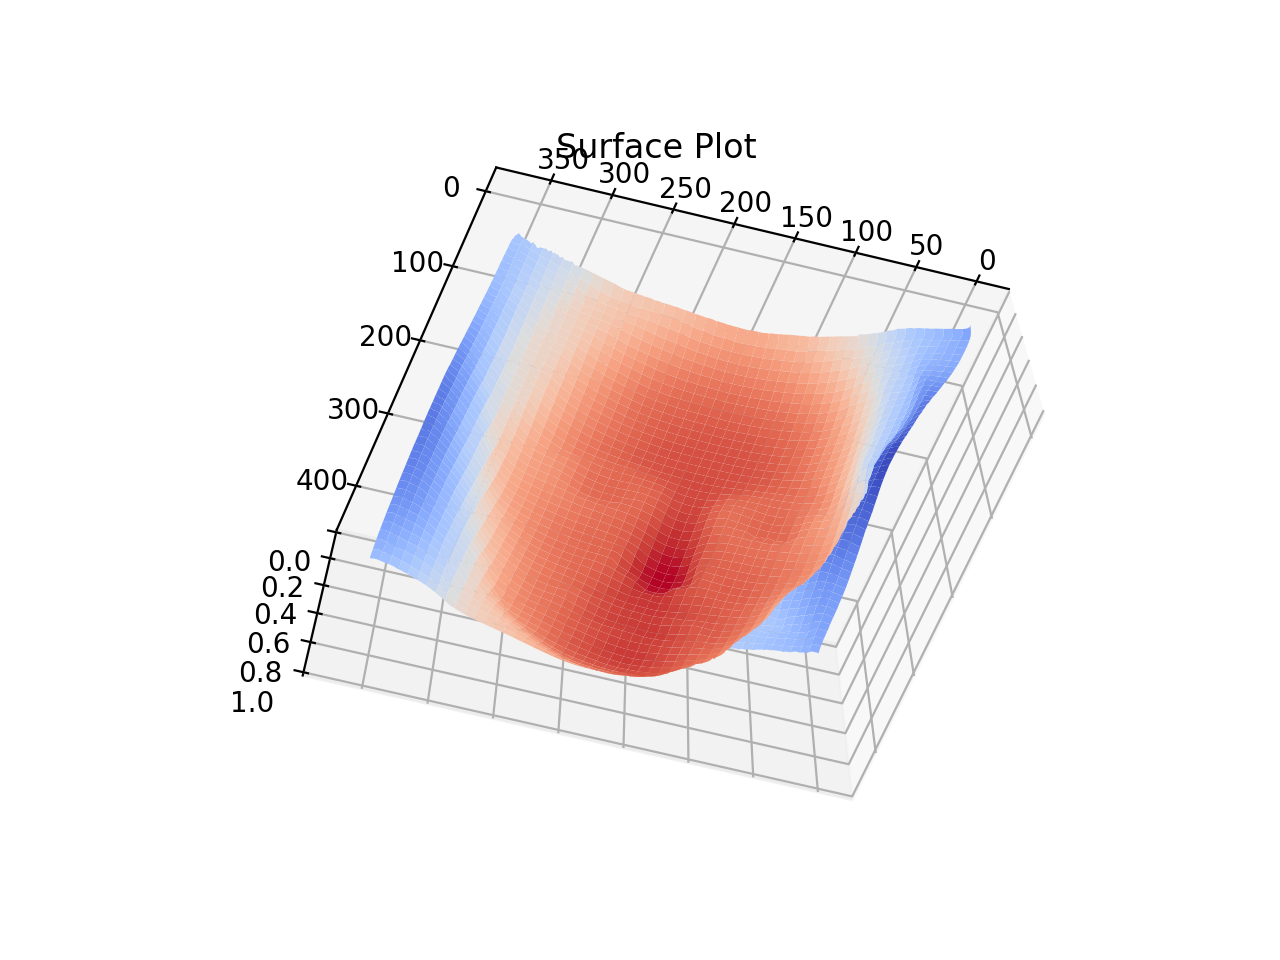
\includegraphics[width=0.3\textwidth]{results/q2e_3.png}}
\caption{Reconstructed results}
\end{figure}

Noticed that with enforce integrability the results look much better.

\paragraph{f}~{}

Varying parameters $\mu$, $\nu$, $\lambda$, corresponding surfaces are shown below:
\begin{figure}[H]
\centering
\subfigure[$\mu$ = -0.5]{
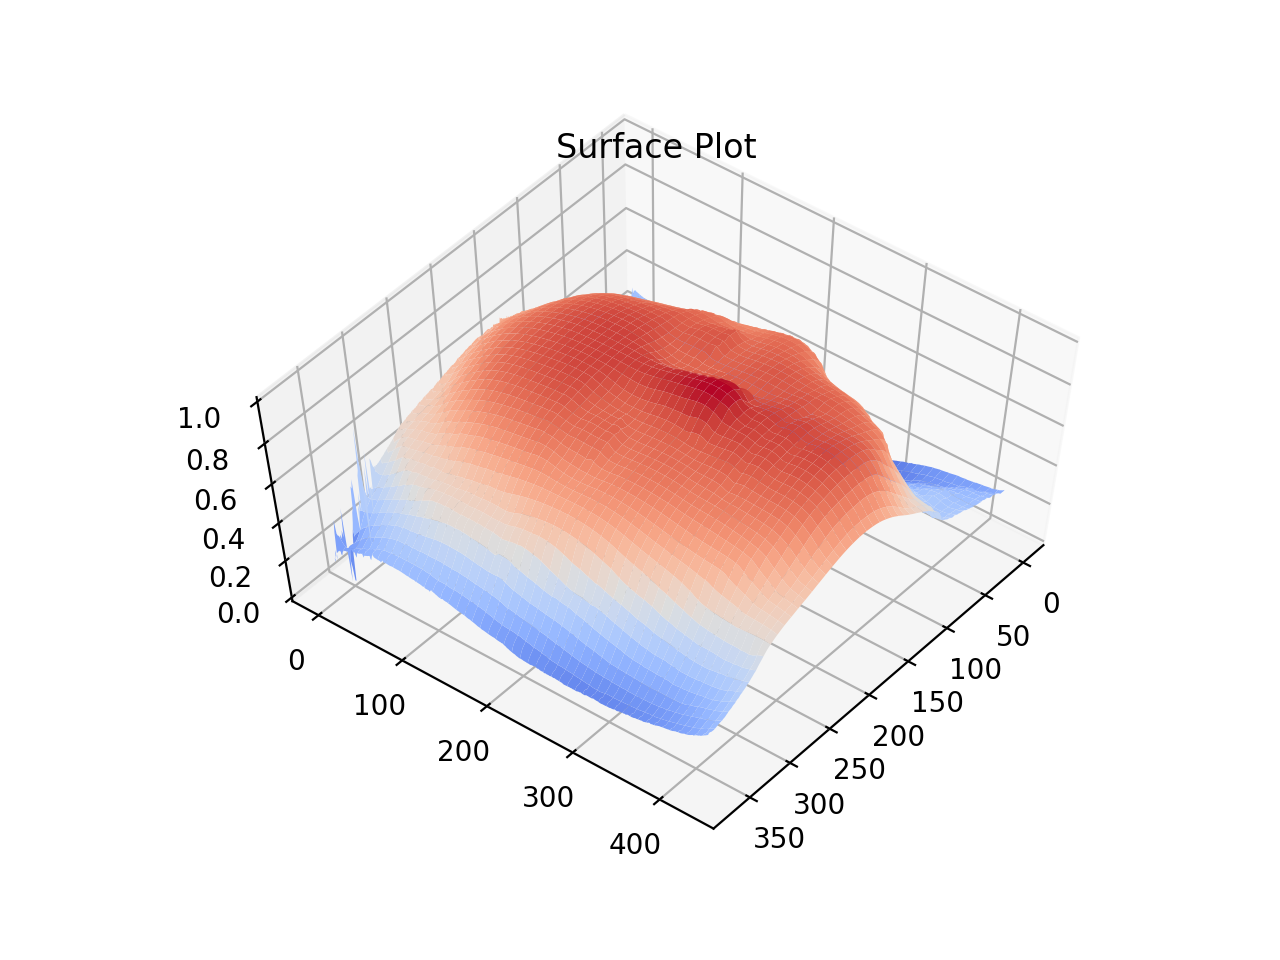
\includegraphics[width=0.3\textwidth]{results/q2f_mu1.png}}
\subfigure[$\mu$ = 0.5]{
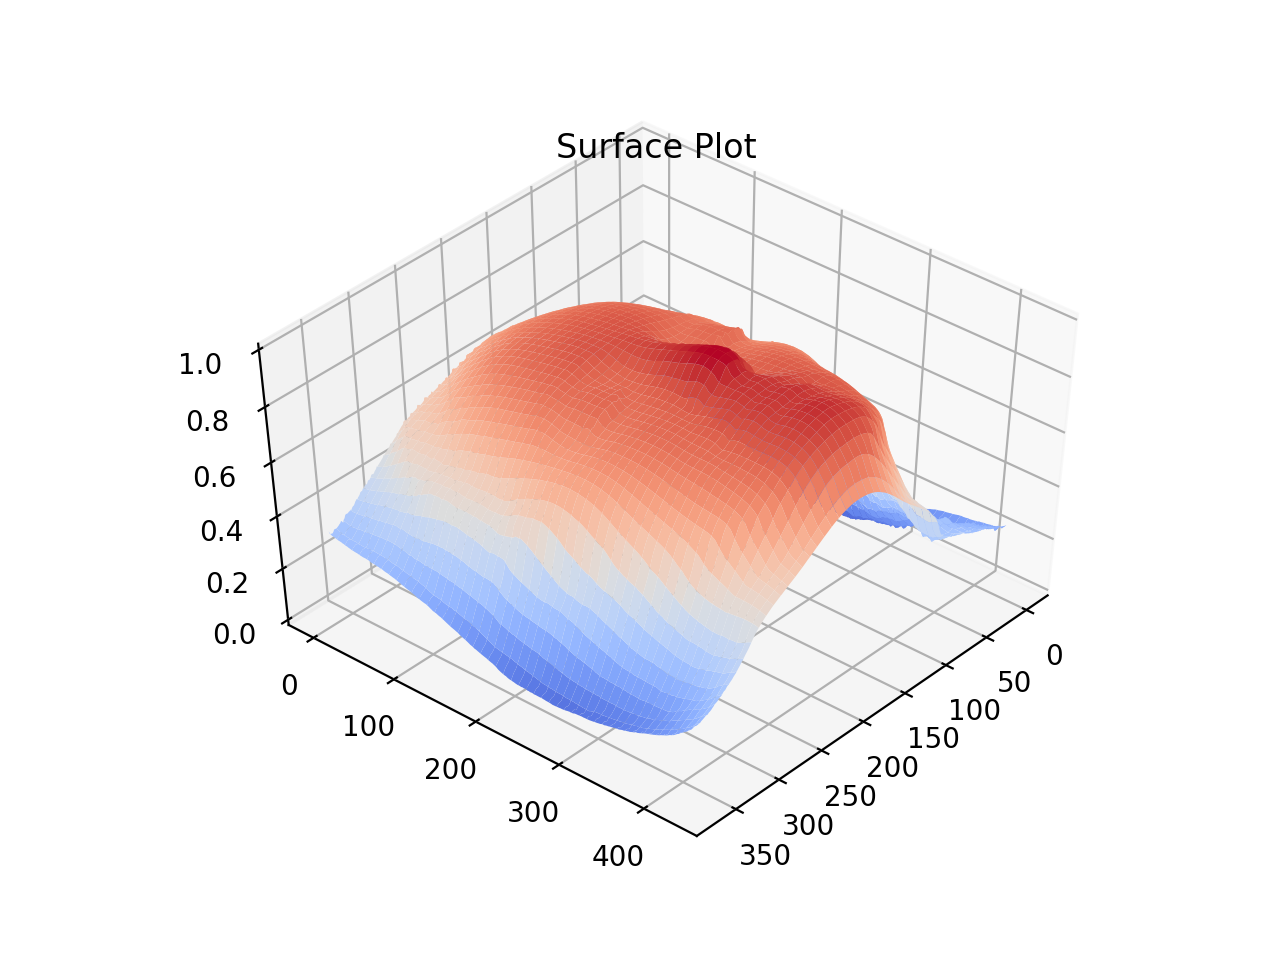
\includegraphics[width=0.3\textwidth]{results/q2f_mu2.png}}
\subfigure[$\mu$ = 1]{
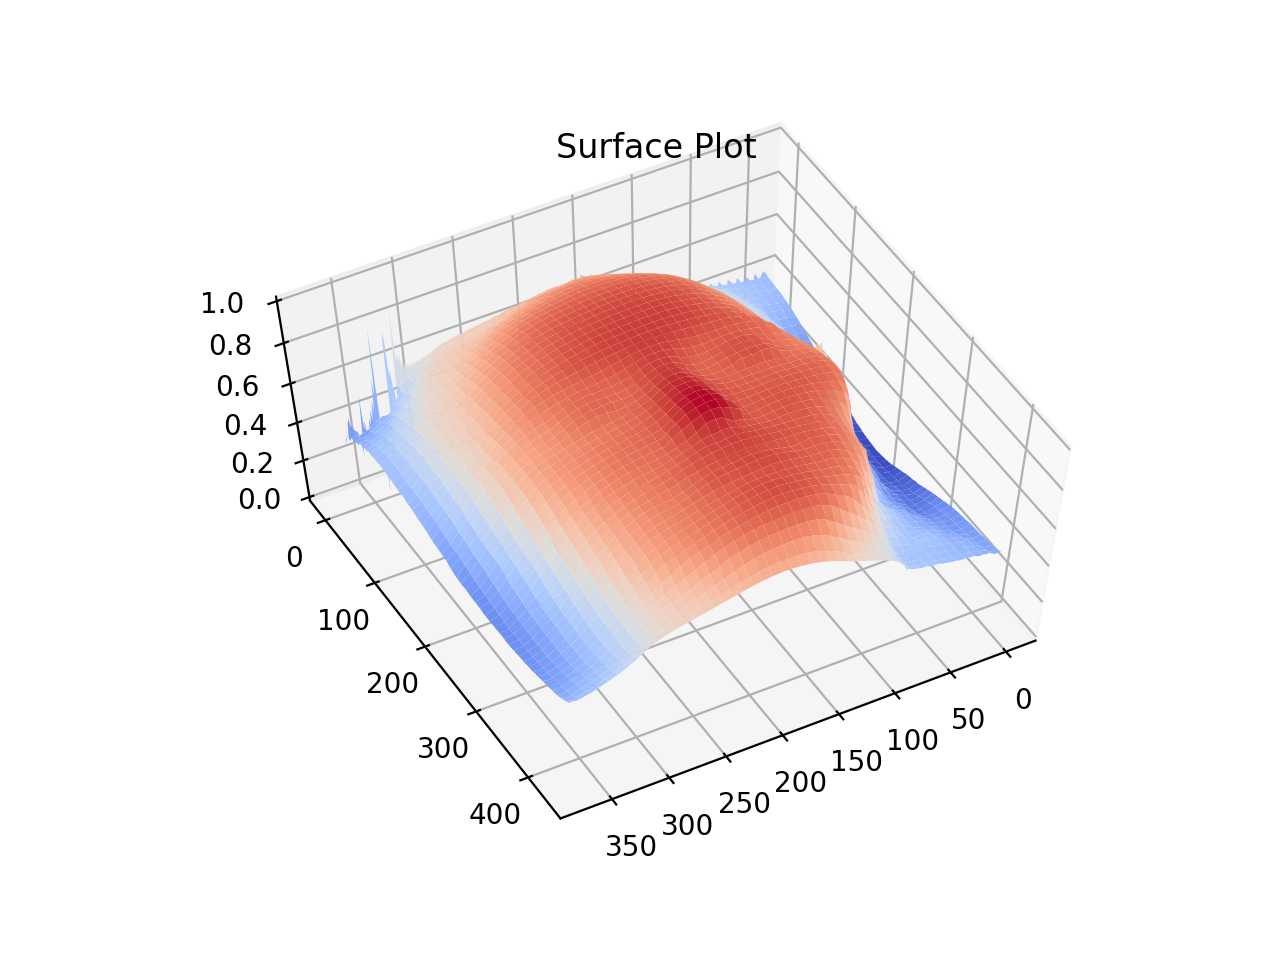
\includegraphics[width=0.3\textwidth]{results/q2f_mu3.png}}
\caption{Varying $\mu$}
\end{figure}

Changing $\mu$ in a small range does not affect the reconstruction much.

\begin{figure}[H]
\centering
\subfigure[$\nu$ = 0.5]{
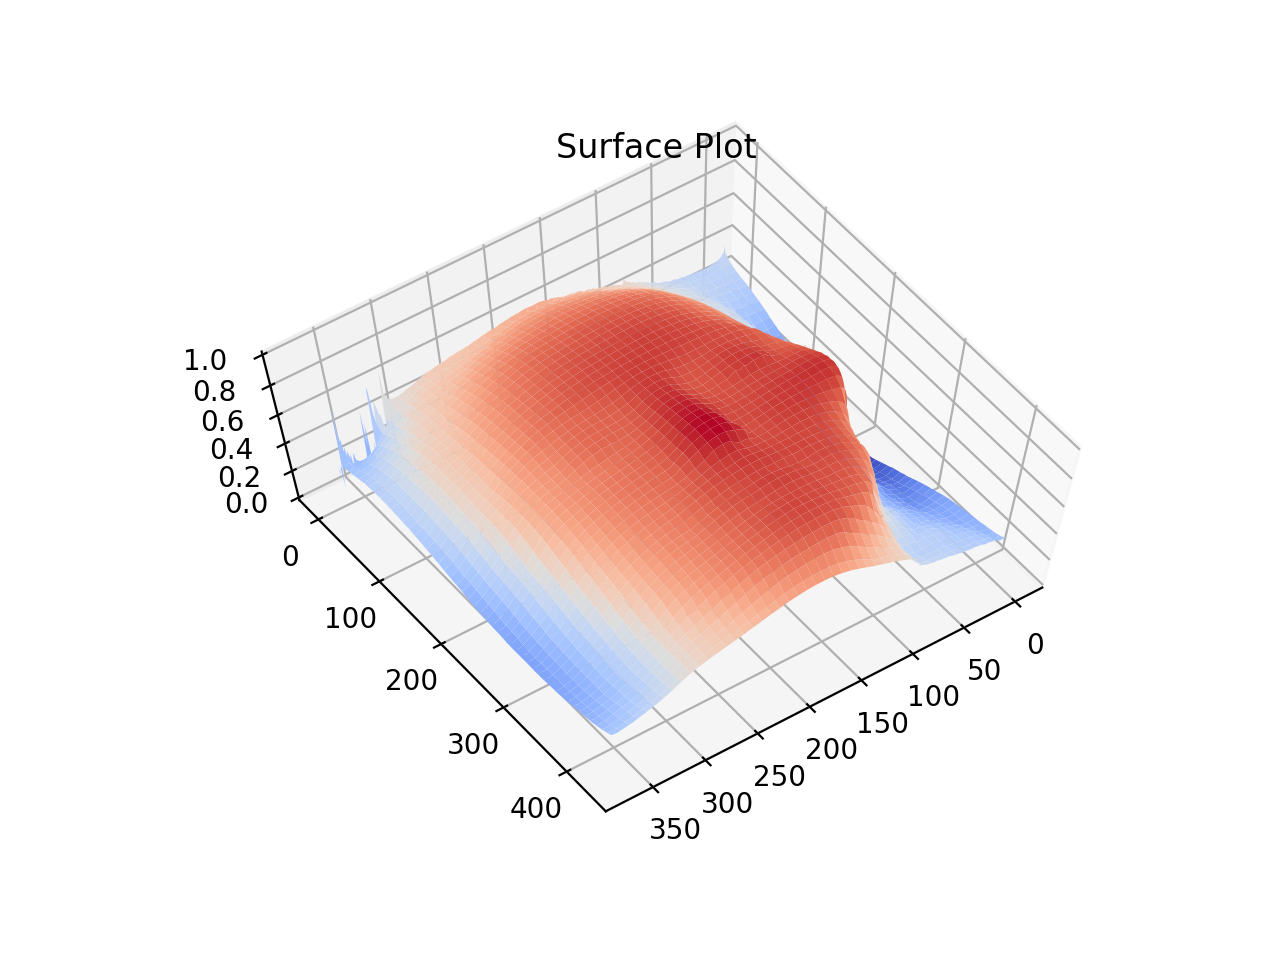
\includegraphics[width=0.3\textwidth]{results/q2f_nu1.png}}
\subfigure[$\nu$ = 1]{
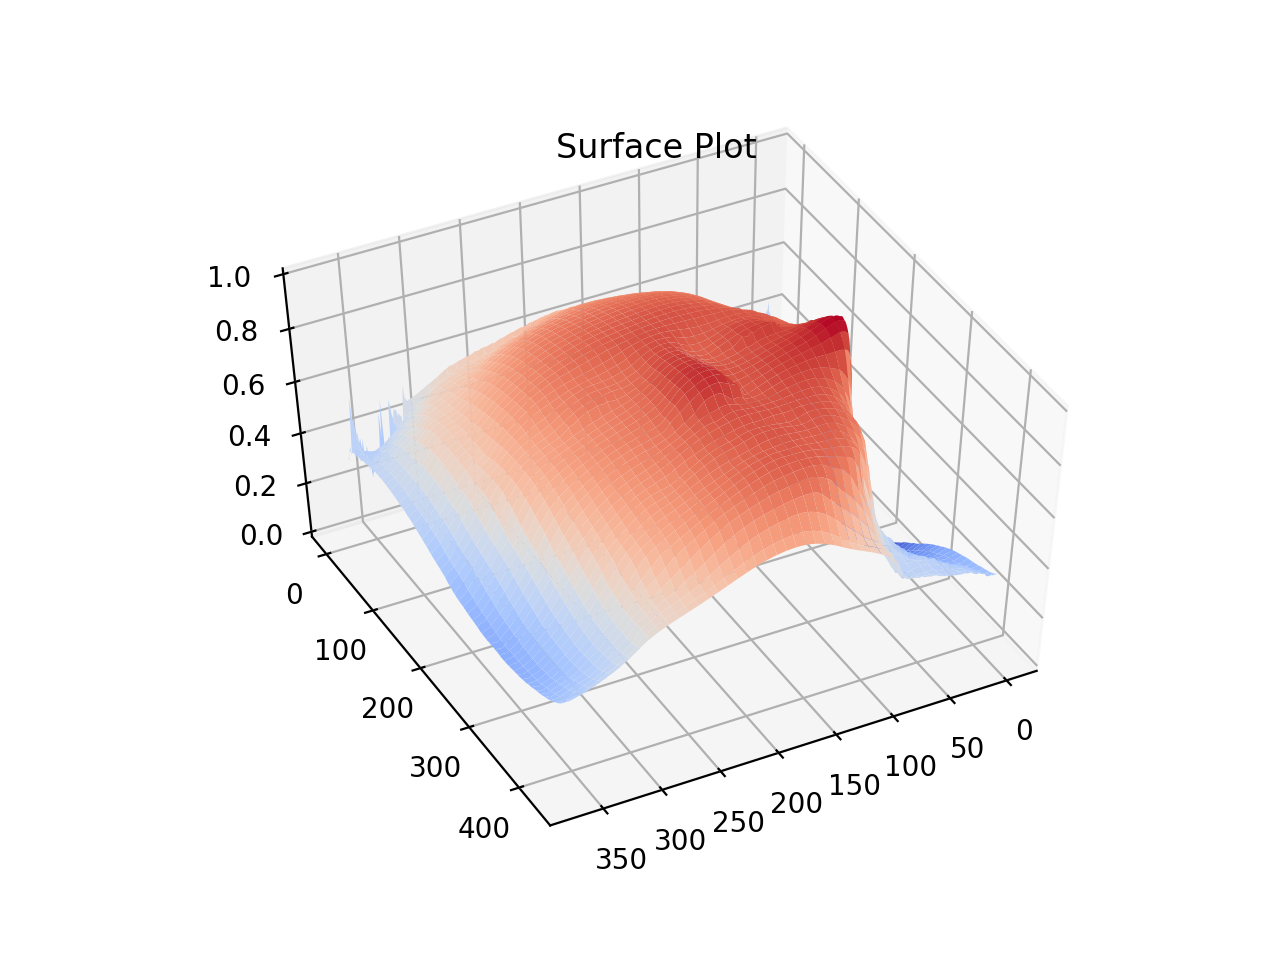
\includegraphics[width=0.3\textwidth]{results/q2f_nu2.png}}
\subfigure[$\nu$ = 3]{
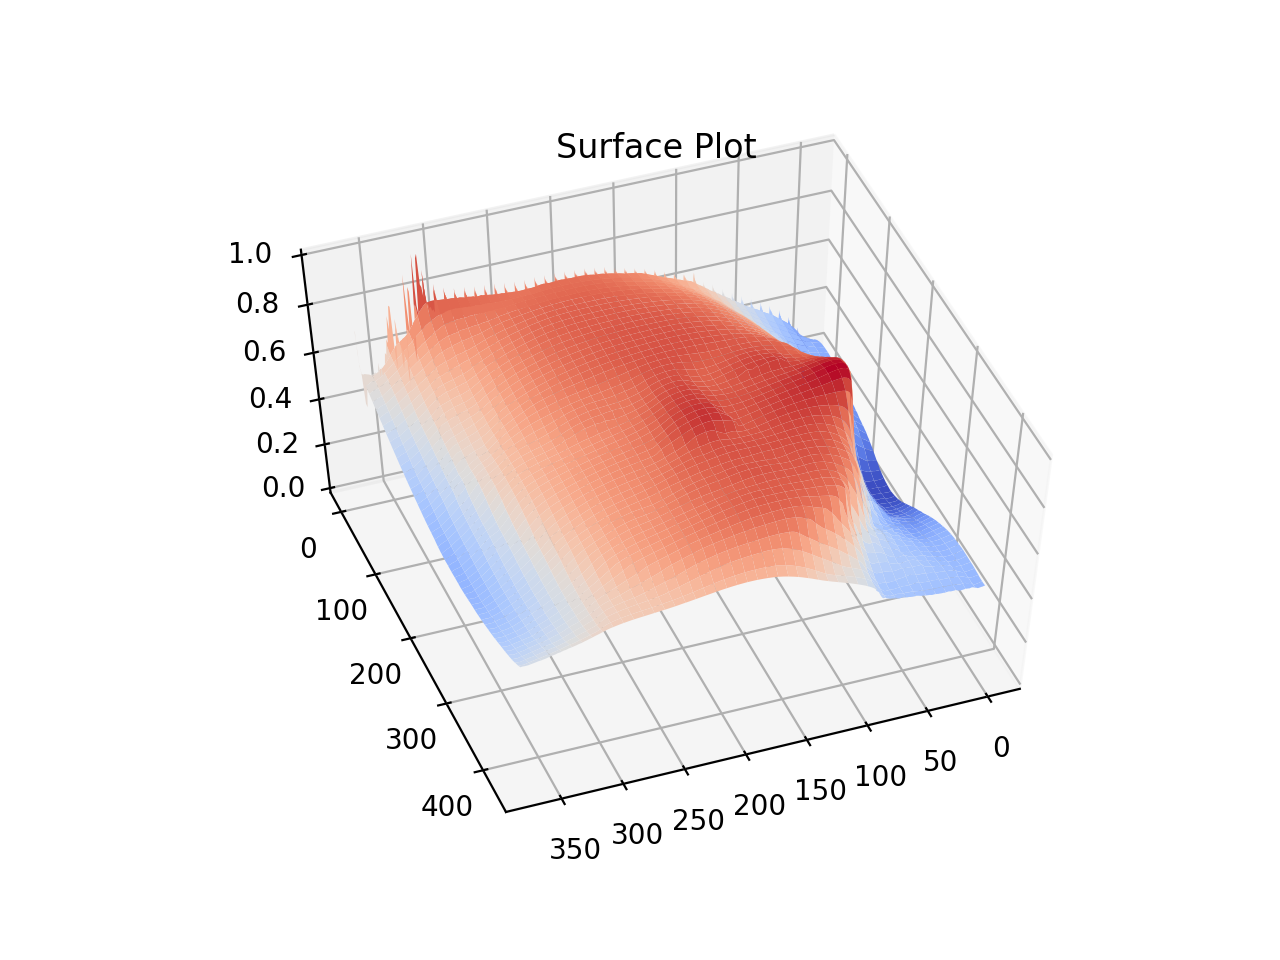
\includegraphics[width=0.3\textwidth]{results/q2f_nu3.png}}
\caption{Varying $\nu$}
\end{figure}

Noticed that increasing $\nu$ would stretch one side of the face, which indicates the increase of gradients.

\begin{figure}[H]
\centering
\subfigure[$\lambda$ = -1]{
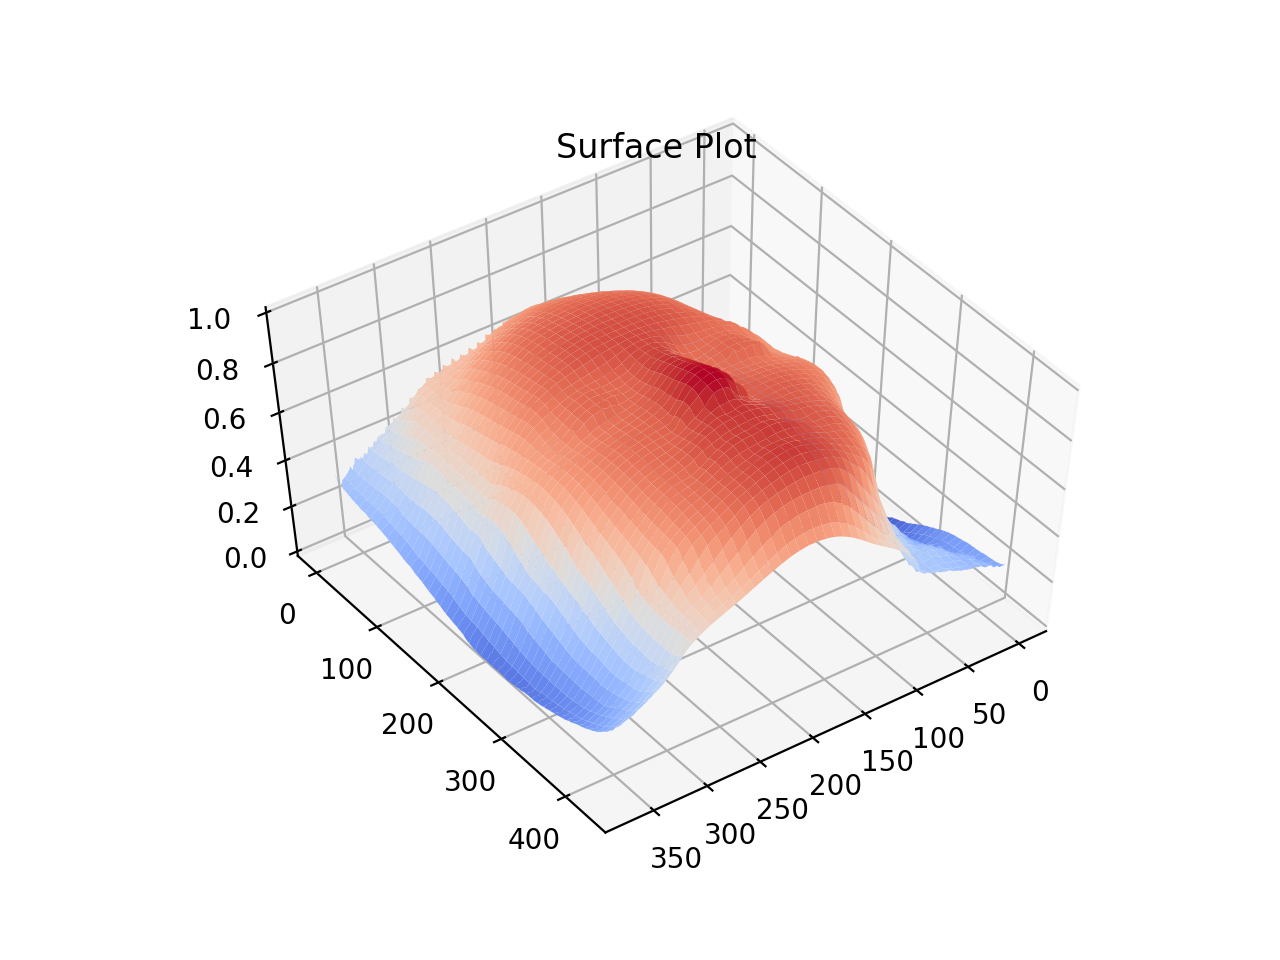
\includegraphics[width=0.3\textwidth]{results/q2f_lambda1.png}}
\subfigure[$\lambda$ = 1.5]{
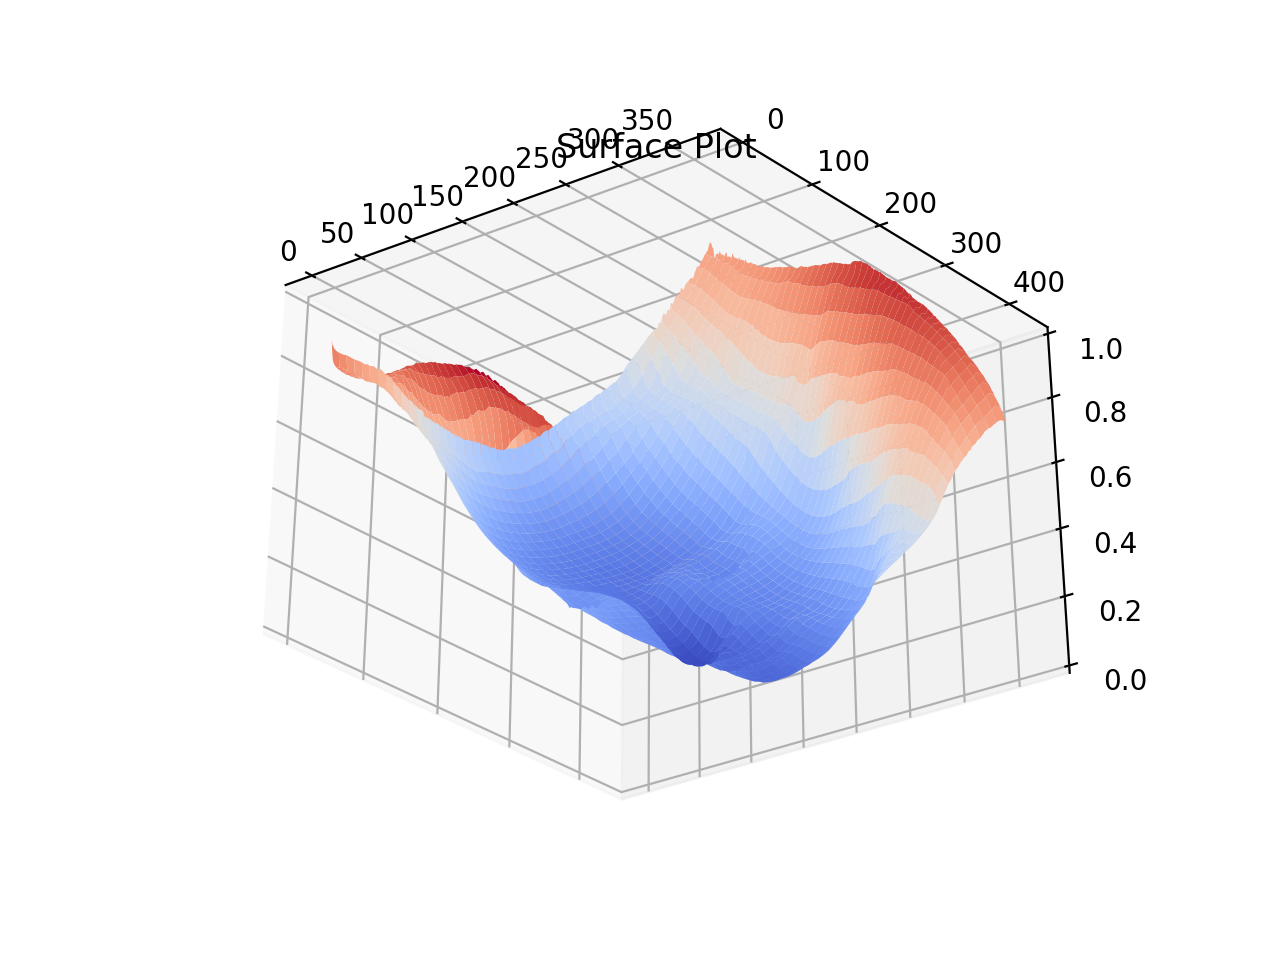
\includegraphics[width=0.3\textwidth]{results/q2f_lambda2.png}}
\subfigure[$\lambda$ = 3]{
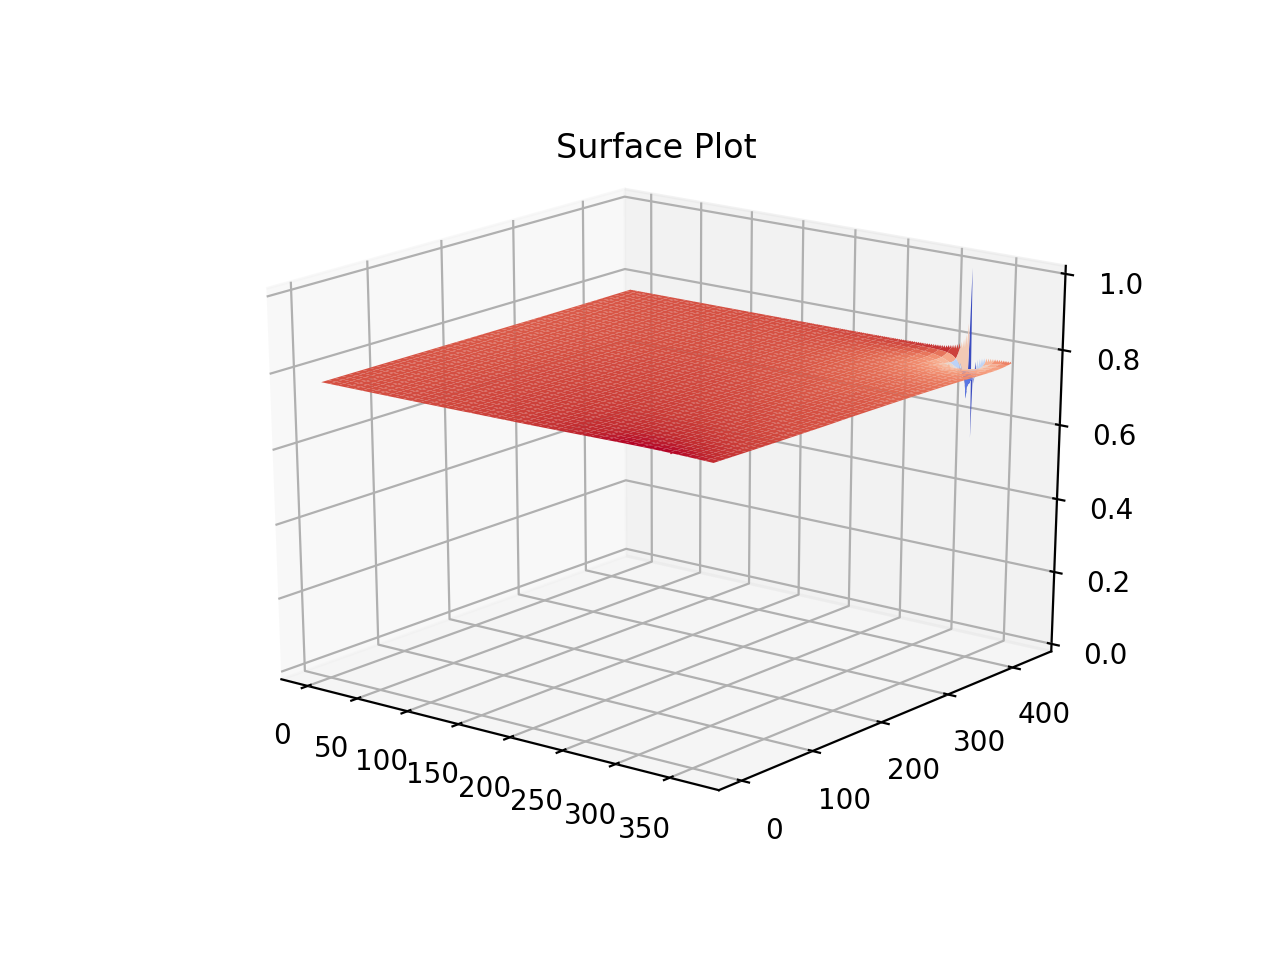
\includegraphics[width=0.3\textwidth]{results/q2f_lambda3.png}}
\caption{Varying $\lambda$}
\end{figure}

Noticed that with large $\lambda$ the reconstruction became a flat area, which may be gradients vanished.

\paragraph{g}~{}

To make the estimated surface flattest, I would choose large $\lambda$ and set $\mu$ and $\nu$ to zero.

\paragraph{h}~{}

Acquiring more pictures from more lighting directions would help in finding a better reconstruction but it could be computational consuming.

\section{Homework Feedback}

This homework is a pretty well designed one, since it contains a lot basic knowledge about photometric stereo, but the coding part is not as complicated as I have expected, each coding question could be done in several lines. I guess it's probably due to the virus issue, but if you want to keep this homework in following semesters, I think more coding work could be included in order to get more hand-on experience.

But the shortcoming is that the description for some theory questions like 1d, 1h is not explicit enough, it may requires more additional information to help understanding the questions, and too much details which haven't been covered in class has appeared in homework, which would cause more difficulty in understanding theory questions.

\end{document}
